\chapter{Error propagation in depletion calculations}
In the \gls{MC} depletion analyses, the uncertainties on predicted isotopic 
composition are caused by two primary factors: stochastic uncertainty in 
the computed flux and uncertainty in the nuclear data (cross sections, fission 
yields, decay constants). In \gls{MC} reactor physics software, the stochastic 
uncertainty of single burnup step is superposed with errors, propagated 
throughout calculation from previous steps. Over time, these errors 
accumulate, and cumulative error in the predicted number density might be 
significant for the lifetime-long fuel depletion calculations.

Takeda \emph{et al.} first proposed a method to evaluate uncertainty of the 
number density in the \gls{MC} simulations applying the sensitivities of the 
burnup matrix to cross sections and number densities. Takeda and colleagues 
propagated covariances of the cross sections and obtained the number 
density uncertainty due to the cross section error of about 4\% for major 
heavy isotopes ($^{235}$U, $^{239}$Pu, $^{241}$Pu) after 400-day 
\gls{MC} burnup calculation for homogeneous model of fast reactor. Notably, 
the number density uncertainty due to the stochastic error in MCNP was 
much lower: about 0.03\% for $^{241}$Pu, 0.02\% for $^{235}$U, and $<0.004$\% 
for $^{238}$U. The Takeda model showed that statistical error contribution to 
the total error in number densities of major heavy isotopes and \glspl{FP} is 
less than 1\% \cite{takeda_estimation_1999}. Finally, substantial neutron 
population ($N$) increase can theoretically reduce the stochastic error to 
zero but it is enormously expensive due to slow convergence ($O(\sqrt{N})$) of 
Monte Carlo method.

Garcia-Herranz \emph{et al.} used MCNP and in-house code ACAB to analyze the 
uncertainties on the nuclide inventory based on random samplinq technique for 
single, spherical fuel element (``pebble") contained coated PuO$_2$ fuel 
particle. The random sampling or ``brute force" method is the multi-step 
scheme of stochastic neutronics and depletion calculation could be considered 
as a single process with (nuclear data) and output (final number densities). 
Authors performed a simultaneous random sampling of all the cross 
sections\footnote{Authors assumed that the influence of uncertainties in decay 
constants, fission yields and other input parameters are negligible.} 1000 
times and obtained the distributions of the isotopic inventory. Relative error 
of the final number density for 1200-day fuel cycle (800 MWg/kgHM burnup) due 
to cross section uncertainties was reported in range from 7\% (for $^{244}$Pu) 
to 46\% (for $^{242}$Pu) and found to be independent of neutron history size. 
In contrast, similar characteristic but only due to stochastic error for 
reasonably large neutron history was less than 0.15\% 
\cite{garcia-herranz_propagation_2008}. Thus, random sampling Monte Carlo 
results by Garcia-Herranz \emph{et al.} agreed with Takeda statement that 
nuclear data is the major source of uncertainty; stochastic error contribution 
to the total nuclear density error is negligibly small ($<1$\%) and might be 
reduced to almost further by substantially increasing neutron histories.

In similar vein, Radaideh \emph{et al.} used SCALE 6.2 
\cite{rearden_scale_2018} to quantify the uncertainty in nuclide concentration 
in \gls{BWR} 10$\times$10 assembly due to uncertainties in neutron cross 
sections, fission yield, and decay data \cite{radaideh_uncertainty_2018}. The 
Radaideh model used 56-group covariance library in deterministic code TRITON 
(2D) depletion calculations and, hence, introduced no stochastic error in the 
flux calculations. That work used 500 random samples in 1174-day TRITON 
depletion calculation and reported number density uncertainty between 0.14\% 
for $^{238}$U and 6.56\% for $^{238}$Pu \cite{radaideh_novel_2019-1}. This 
approach
benefits from Sampler module available in the SCALE package and 
can be used by SCALE users across the world.

All listed research efforts studied simplified, pin-cell or single-assembly 
models of conventional \gls{LWR} and considered nuclear data uncertainty for 
following elements: hydrogen, oxygen, zirconium, uranium, and plutonium. The 
nuclear data for these elements have relatively low uncertainty because it was 
measured many times for myriad weapon and non-weapon applications. However, 
the \gls{TAP} \gls{MSR} and many other designs rely on other elements such as 
lithium and fluorine which have relatively high cross section covariances. 
Effect of $^6$Li, $^7$Li, and $^{19}$F nuclear data uncertainty on final 
isotopic composition uncertainty was never studied before. This chapter seeks 
to estimate the uncertainties on predicted isotopic composition for the 
\gls{TAP} \gls{MSR} during lifetime-long depletion simulations.

In this chapter, the uncertainty in the fuel salt composition will be 
investigated for two different sources of uncertainty separately. The 
uncertainty in the nuclides inventory due to the transport problem statistical 
error is evaluated using random sampling technique using Serpent Monte Carlo 
code. By changing the code's initial random number seed, the data produce by 
1000 runs is used to investigate statistical error in multiplication factor 
($k_{eff}$) and number density of major isotopes. The uncertainty in depleted 
fuel salt composition due to nuclear data uncertainties - a major part of 
nuclear density uncertainty - is determined using SCALE/Sampler sequence in 
conjunction with TRITON (2D, deterministic code). Uncertainties in nuclear
data (e.g., neutron cross sections, fission yields, decay constants) are 
propagated into the response of interest (fuel salt isotopic composition) by 
generating a large number of samples with perturbed nuclear data. The two 
approaches are demonstrated using the \gls{TAP} reactor model.



\section{Stochastic uncertainty in depleted fuel composition}
This section presents a general approach to uncertainty propagation throughout 
the depletion calculations when using Monte Carlo burnup software. Only 
uncertainties due to the statistical
nature of Monte Carlo neutron transport 
calculation was considered herein. 

\subsection{Methodology of uncertainty propagation by a random sampling}
In nuclear reactors where the changes in the isotopic composition changes the 
neutron flux distribution, a sequence of coupled transport problem and 
depletion calculations should be done. In such coupled calculations, the 
depletion time is divided into a few time intervals. A transport calculation 
is carried out for each time interval and the evaluated reactor rates are then 
used to solve system of the Bateman equations~\ref{eq:bateman} to obtain the 
fuel isotopic composition at the end of the time interval. The goal is not 
only to calculate the isotopic vector at the end of each depletion step, but 
also to estimate stochastic error in the vector due to the statistical nature 
of Monte Carlo neutron transport calculations.

Monte Carlo methods using ``random sampling", which employs a pseudo random 
number generator for sampling probabilities of neutrons from their ``birth" 
until it is either absorbed or escaped \cite{brown_fundamentals_2005}. Each 
neutron history is tallied and when sufficient number of histories are 
accumulated, statistical metrics (mean value, standard deviation) of the 
target parameters are calculated. The \gls{MC} code repeats this process for 
user-defined number of cycles. The first few cycles have poor statistics 
because the \gls{MC} code accumulated insufficient neutron historical data. 
The first few cycles are usually marked ``inactive" and used for source 
convergence only. Therefore, the user must define the number of inactive and 
active cycles to balance the need to assuring source convergence and 
statistical accuracy with computational costs.

Serpent Monte Carlo code calculates the uncertainty of each output parameter. 
During each neutron source cycle, Serpent calculates the sum of the 
collisions, fissions, and other events in that cycle. After all active cycles 
completion, the code computes the statistical mean and associated standard 
deviation based on cycle-specific data. Notably, Serpent estimates the 
uncertainty assuming that all events are independent. Thus, Serpent Monte 
Carlo code does not contain an algorithm that propagates the uncertainties 
from one depletion step to the next. Instead, the estimate uses only data from 
each separate depletion step by itself. Jaakko Lapp\"{a}nen stated, "Error 
propagation in Monte Carlo burnup calculation is a major research topic at the 
moment..." and mentioned unprecedented complexity of the problem 
\cite{leppanen_statistical_2012}.

In order to estimate the variance in the isotopic composition $[N]$ due to 
statistical nature of \gls{MC}, a bash scripting system was developed to run a 
depletion calculation with $S$ burnup steps $M$ times changing nothing except 
the seed value for the random number sequence in the Serpent input 
(Figure~\ref{fig:uq-brute-force}). The multiple ``replication" of each 
depletion sequence produces set of $M$ isotopic concentrations at the end of 
each depletion interval. 
\begin{figure}[hbp!] % replace 't' with 'b' to 
	\centering
	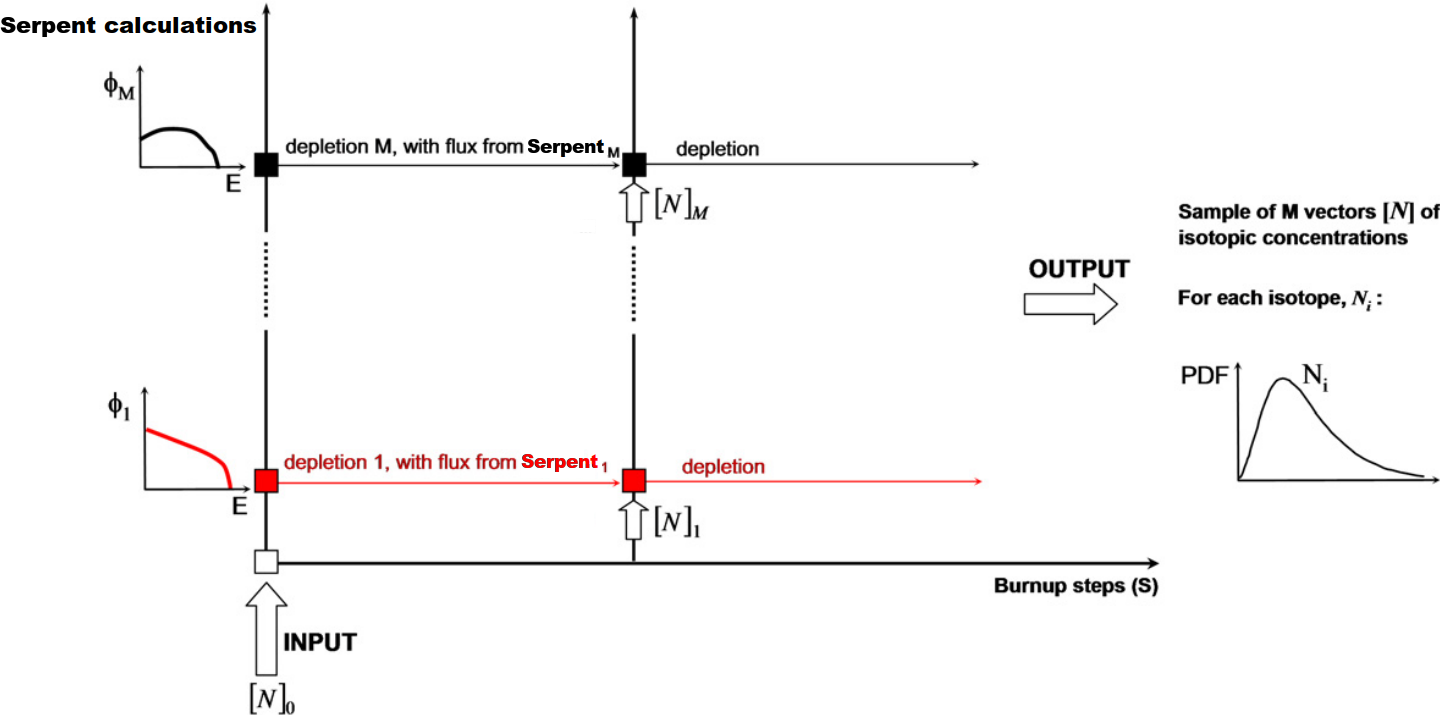
\includegraphics[width=\textwidth]{uq/brute_force_method.png}
	\caption{Principal scheme of random sampling (``brute force") method to 
		propagate uncertainties in final isotopic concentrations (reproduced 
		from 
		Garcia-Herranz \emph{et al.} \cite{garcia-herranz_propagation_2008}).}
	\label{fig:uq-brute-force}
\end{figure}

After running depletion calculations
for all samples, the mean and standard 
deviation of the isotopic concentration can be calculated as
follows
\begin{align}
\overline{N_i} &= \frac{1}{M} \sum_{i=1}^{M} N^{(j)}_i \\
\sigma_{N_i} &= \sqrt{\frac{1}{M-1} \sum_{i=1}^{M} 
(N^{(j)}_i-\overline{N_j})^2}
\intertext{where}
\overline{N_i} &= \mbox{mean concentration of isotope $i$ $[-]$} \nonumber \\
M &= \mbox{number of depletion runs with distinct seed $[-]$} \nonumber \\
N^{(j)}_i &= \mbox{concentration of isotope $i$ in the run $j$ 
$[-]$.} \nonumber
\end{align}



\begin{figure}[hbp!] % replace 't' with 'b' to 
	\centering
	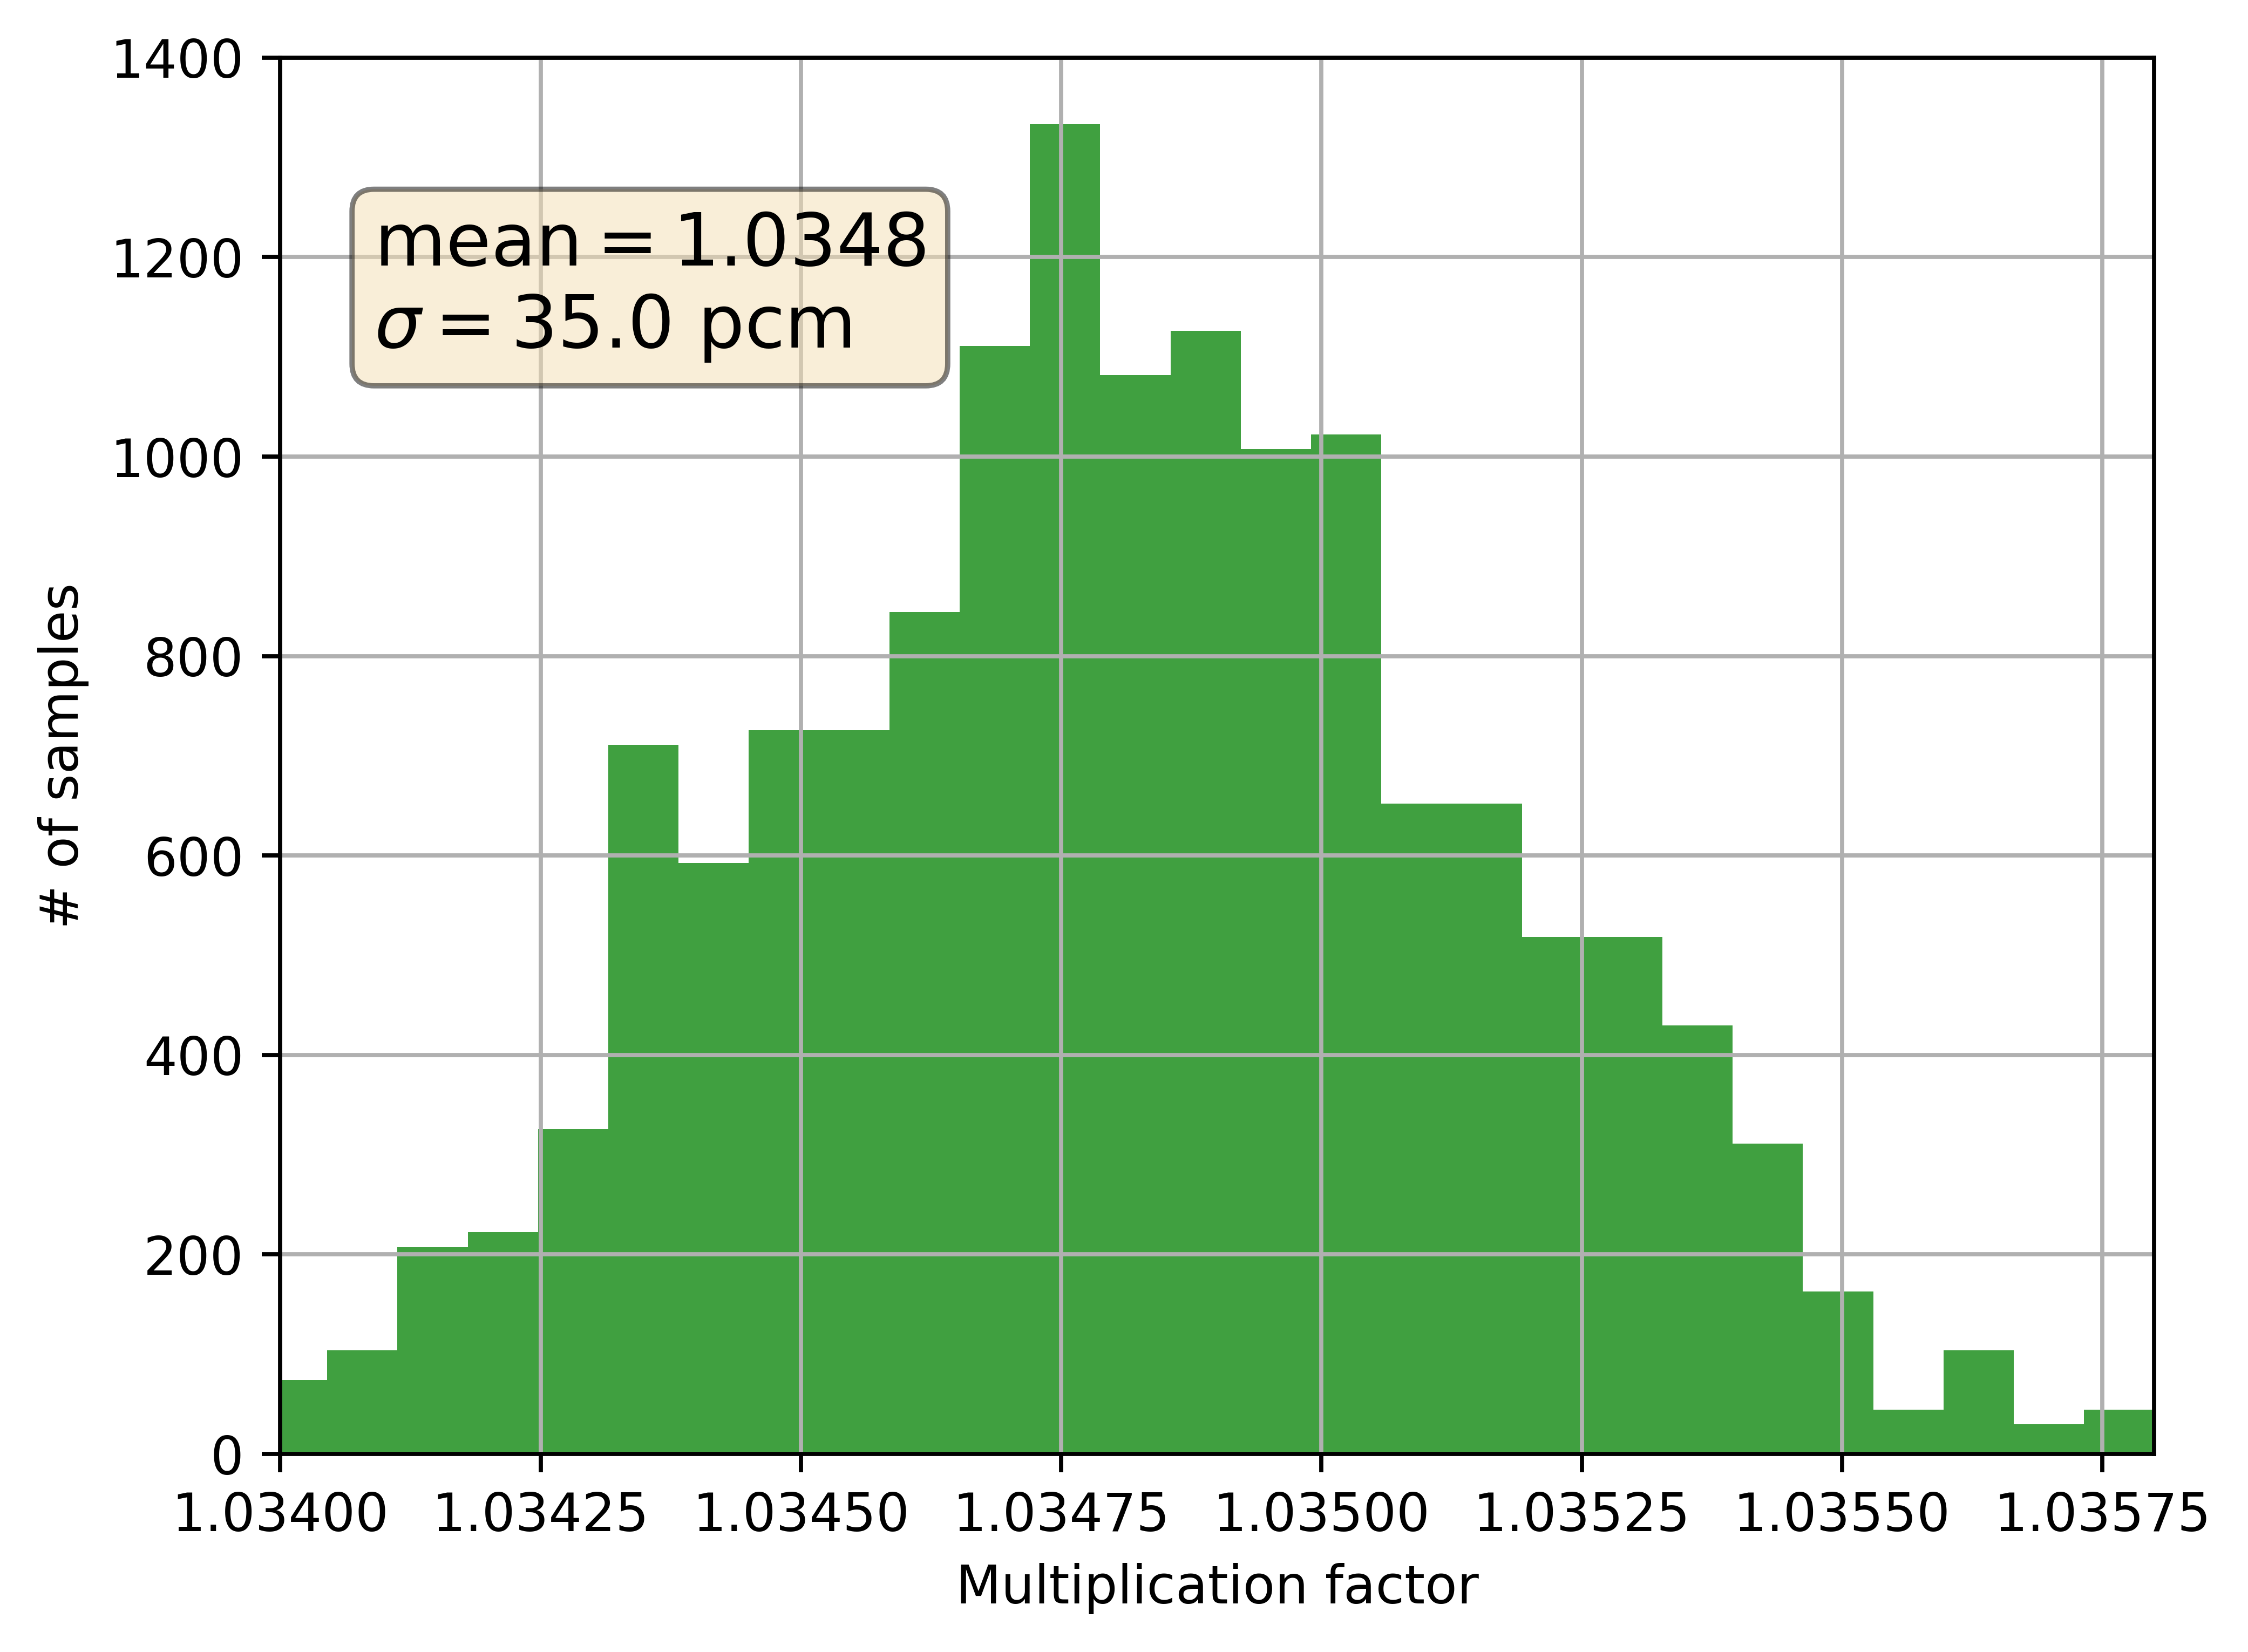
\includegraphics[width=0.8\textwidth]{uq/endf_serpent_keff_boc_for_tap.png}
	\caption{Caption here.}
	\label{fig:11}
\end{figure}
\begin{figure}[hbp!] % replace 't' with 'b' to 
	\centering
	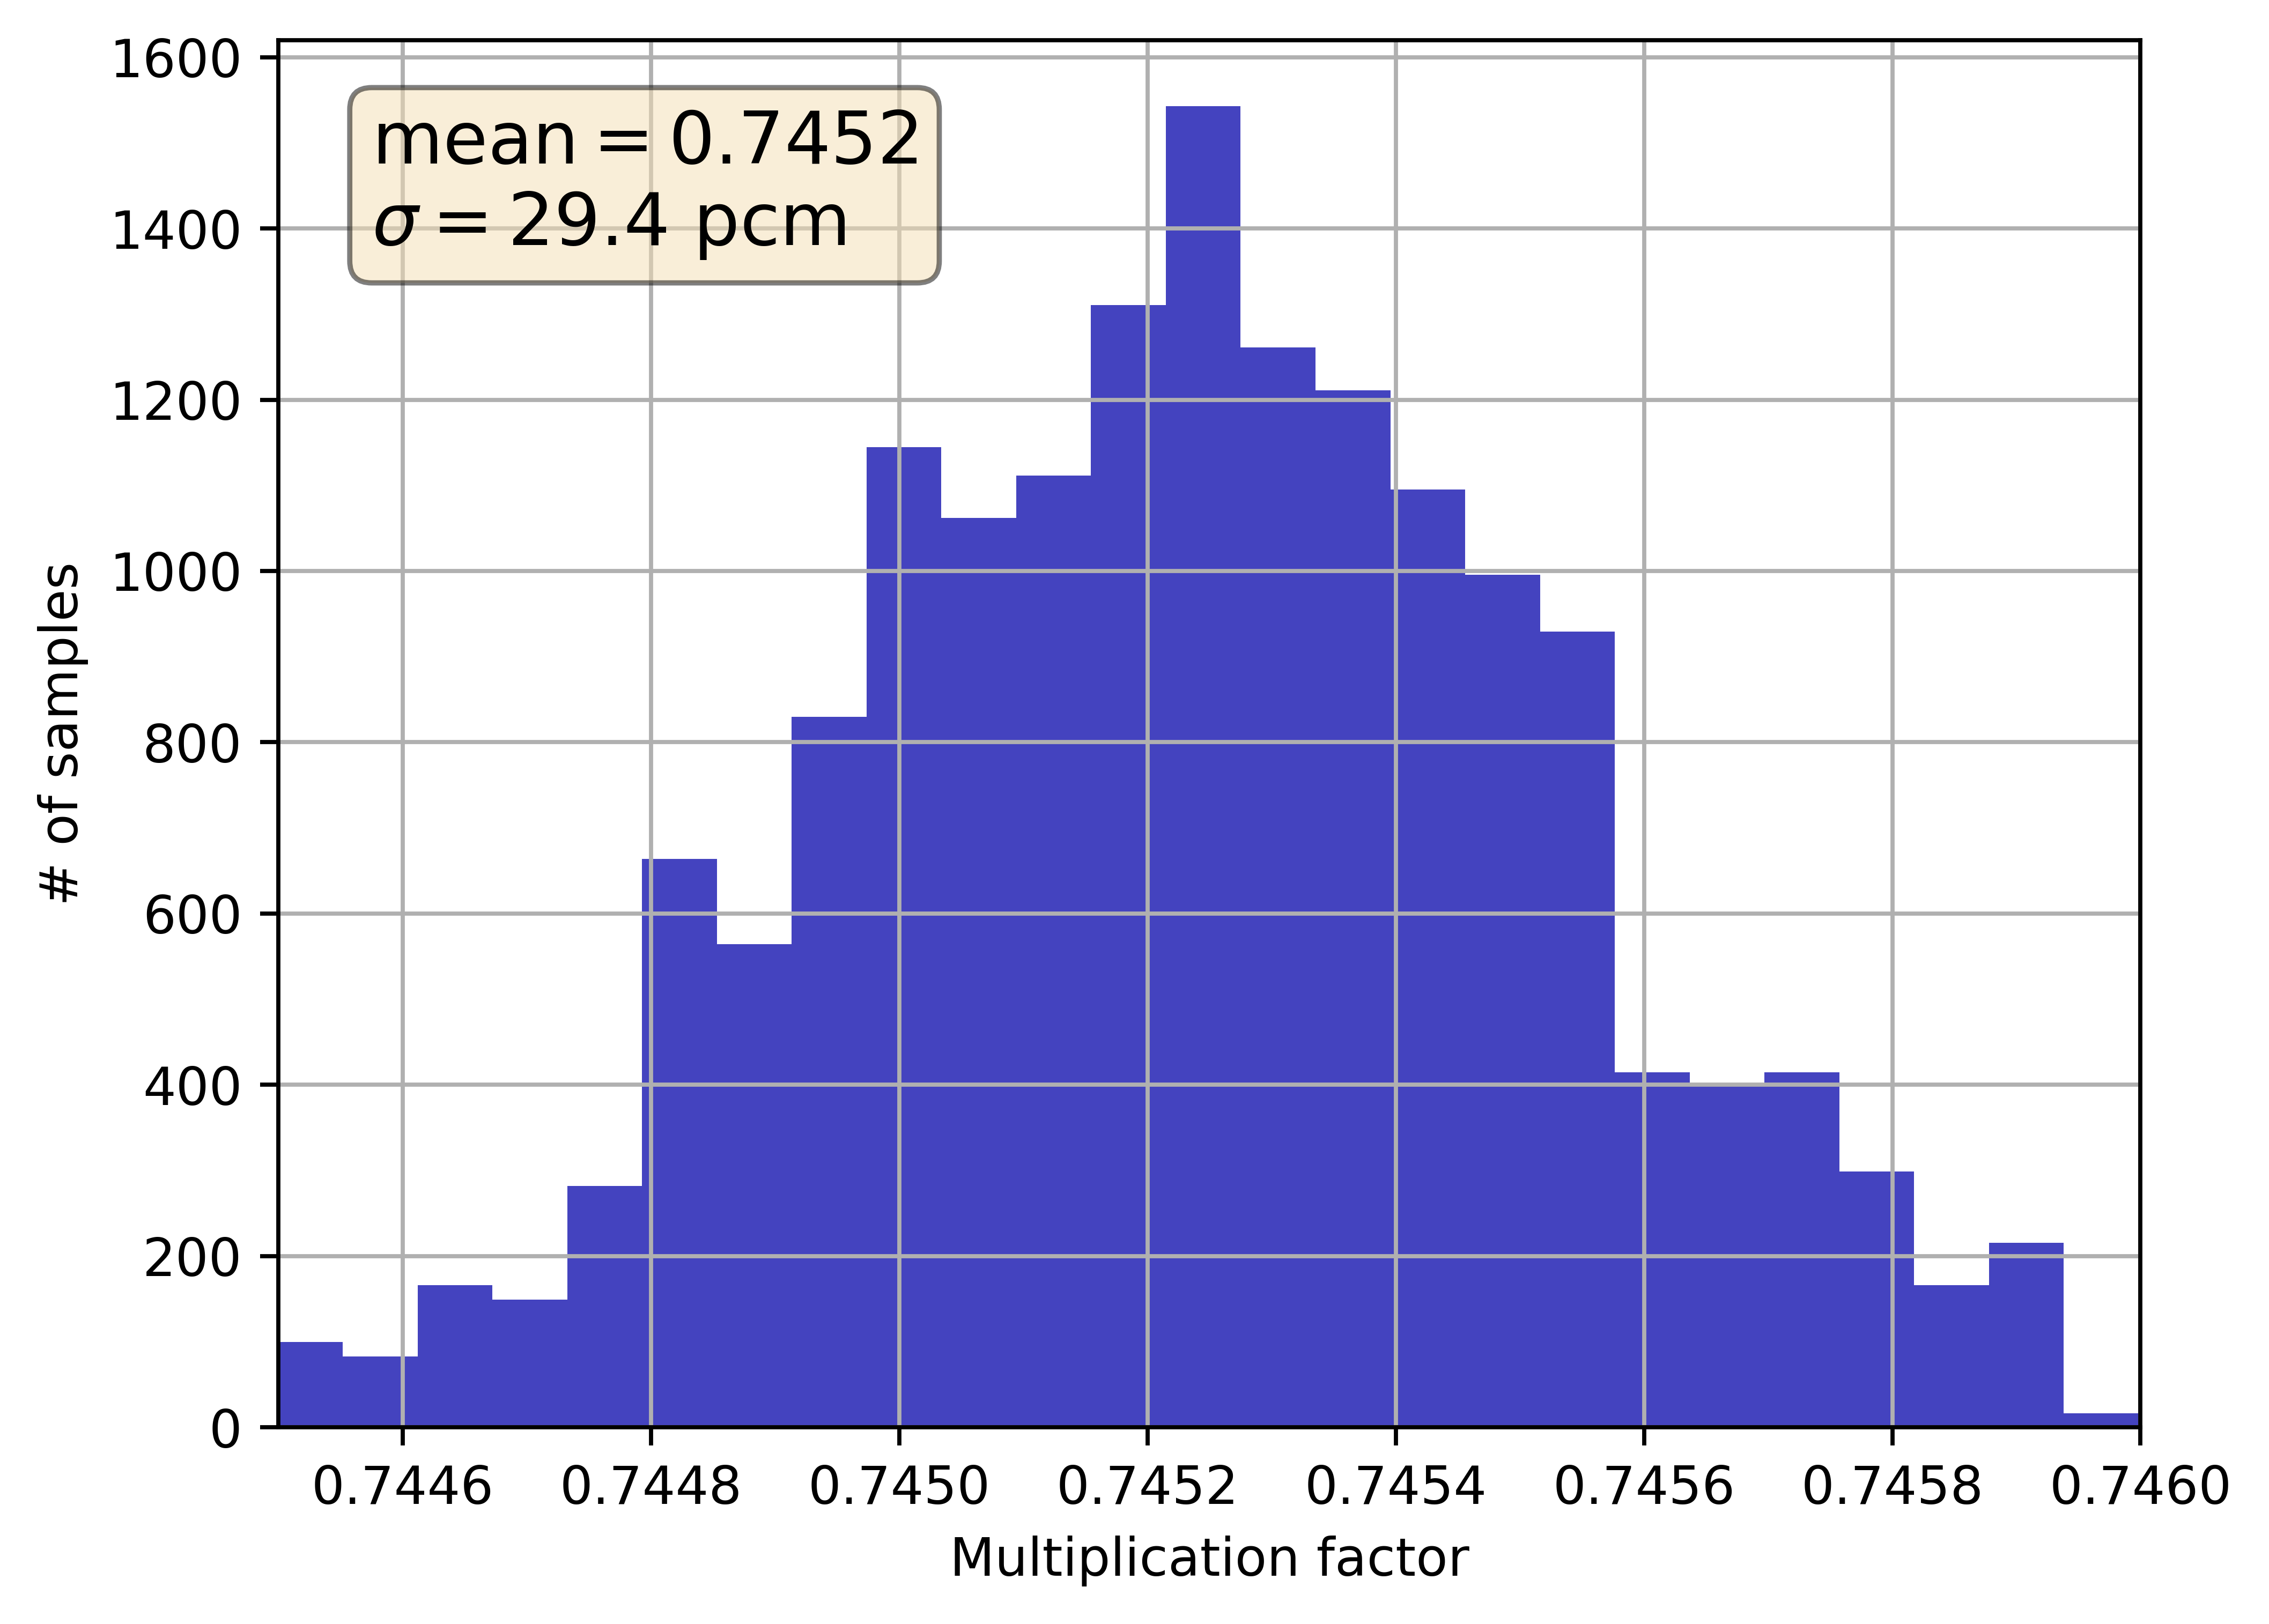
\includegraphics[width=0.8\textwidth]{uq/endf_serpent_keff_eoc_for_tap.png}
	\caption{Caption here.}
	\label{fig:22}
\end{figure}
\begin{figure}[hbp!] % replace 't' with 'b' to 
	\centering
	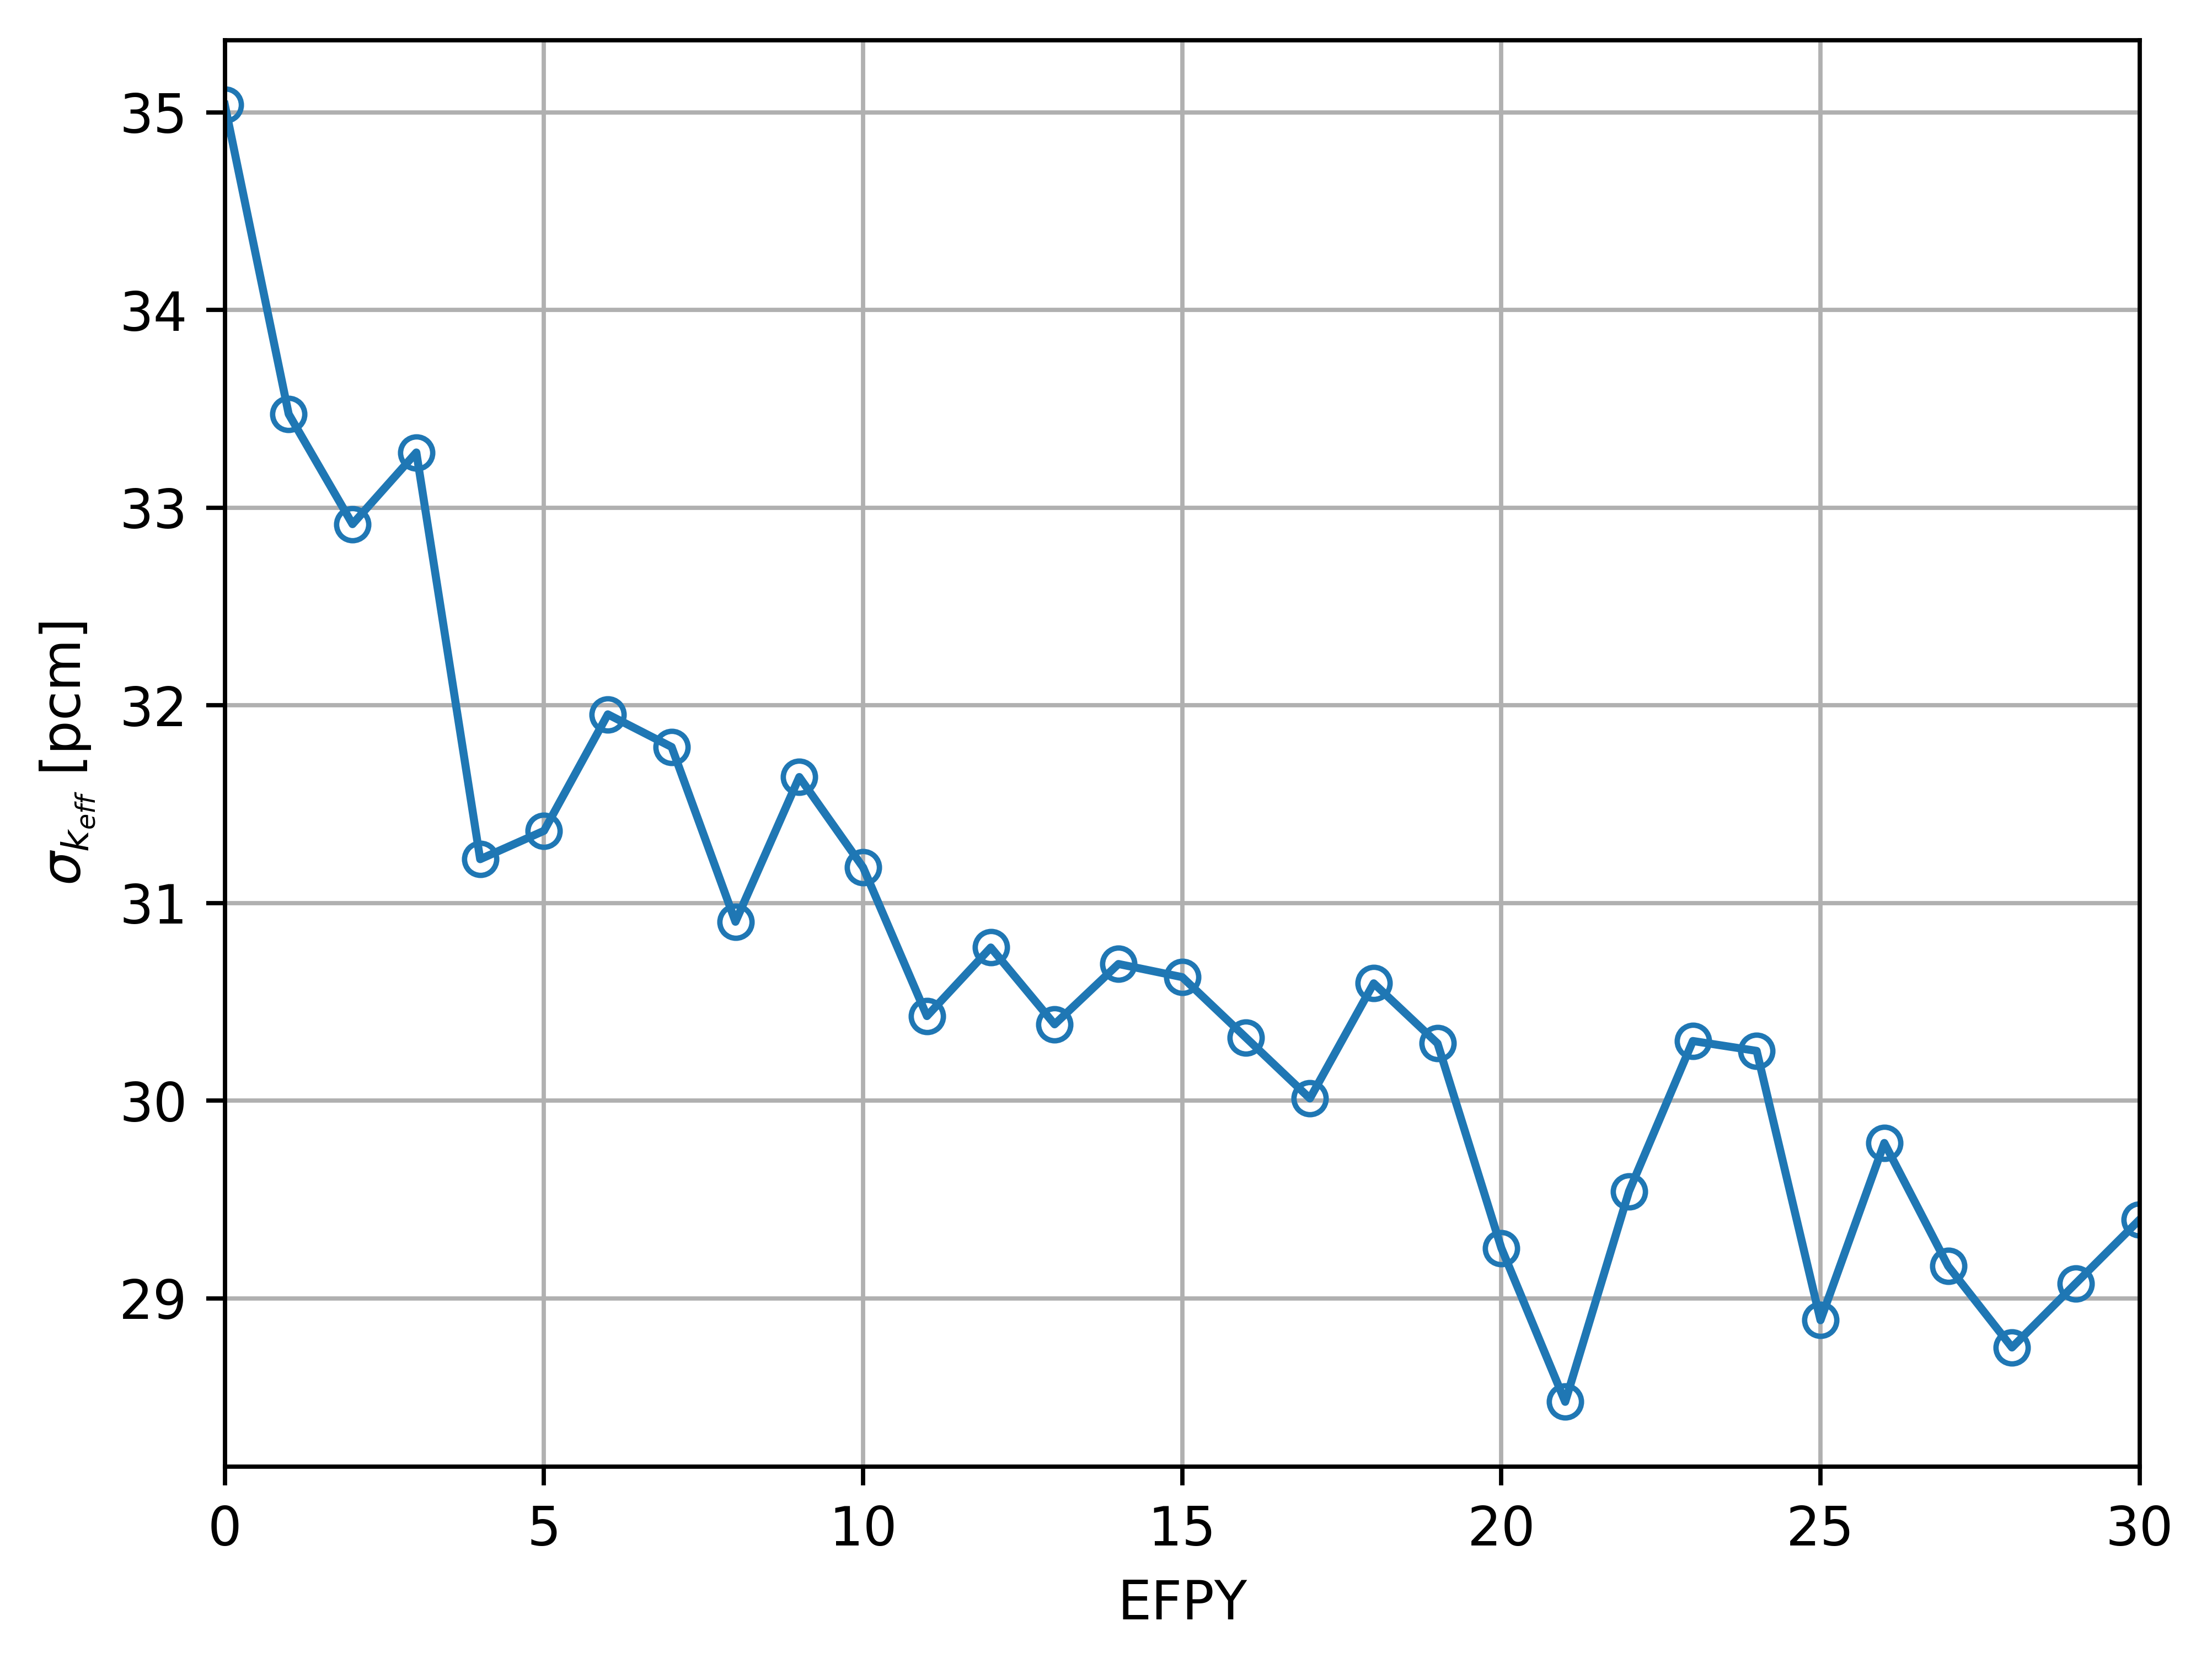
\includegraphics[width=0.8\textwidth]{uq/endf_serpent_keff_dynamics_for_tap.png}
	\caption{Caption here.}
	\label{fig:33}
\end{figure}
\begin{figure}[hbp!] % replace 't' with 'b' to 
	\centering
	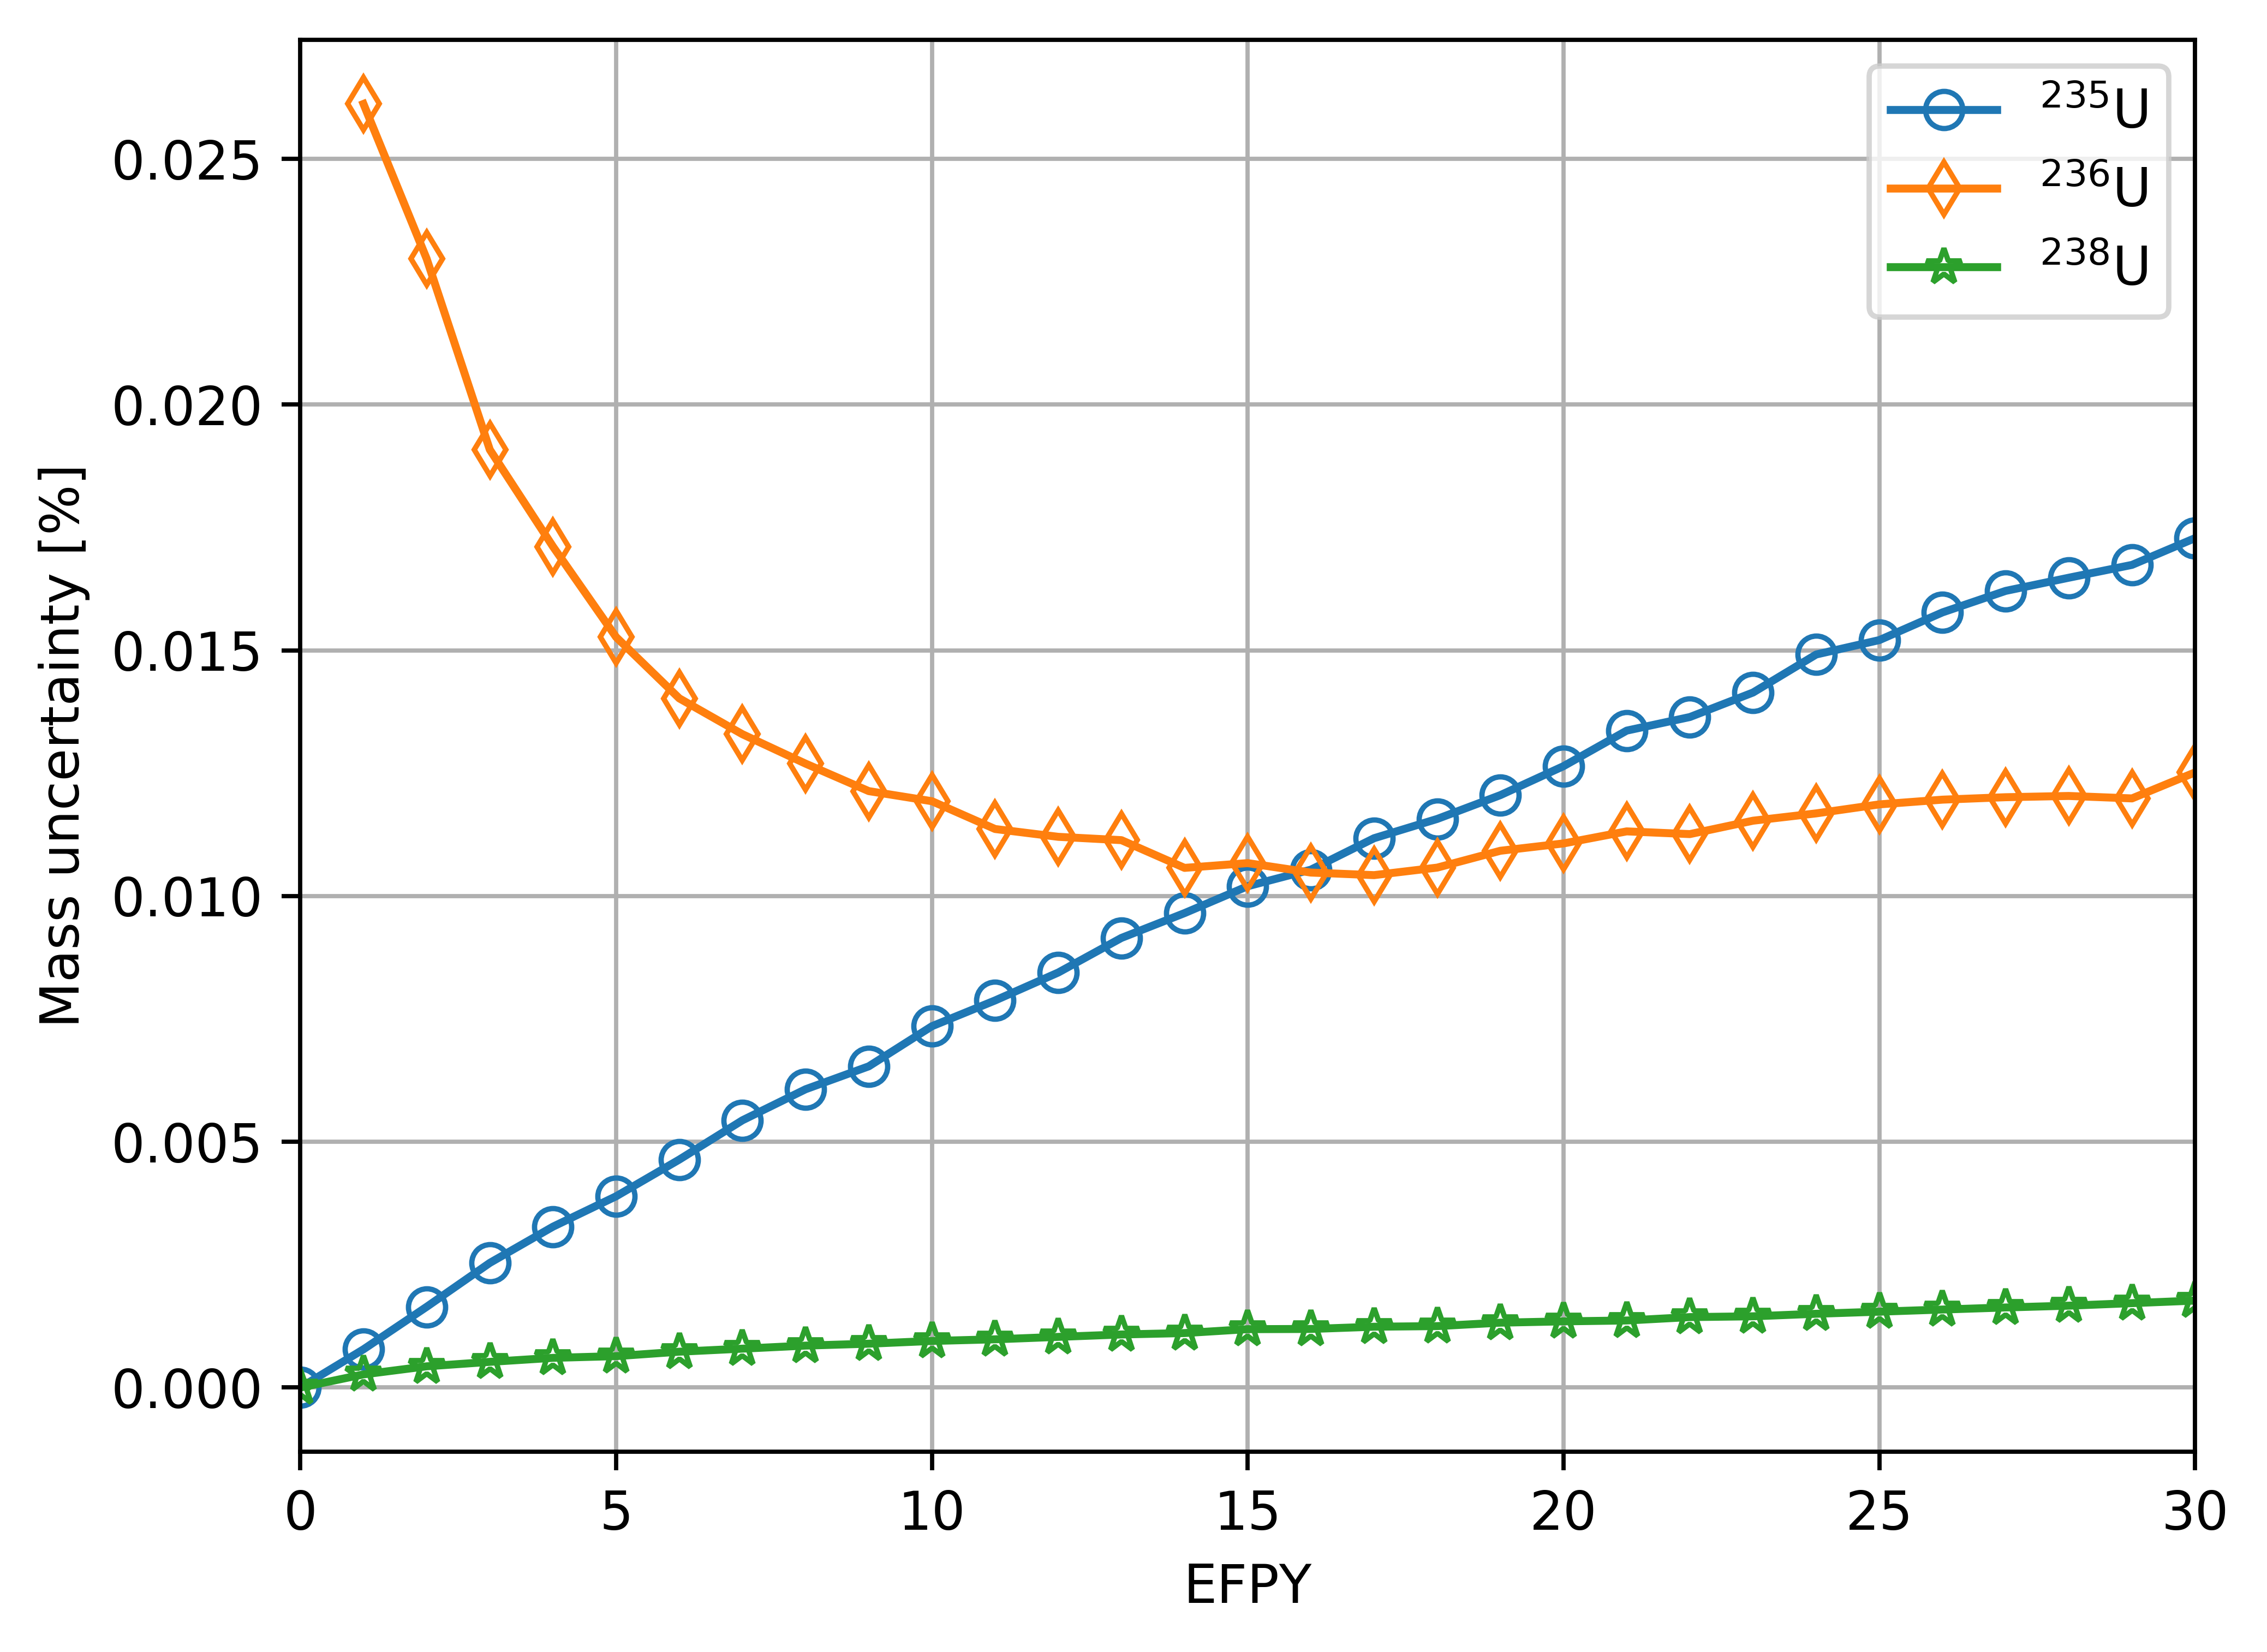
\includegraphics[width=0.8\textwidth]{uq/serpent_mass_std_u.png}
	\caption{Caption here.}
	\label{fig:44}
\end{figure}
\begin{figure}[hbp!] % replace 't' with 'b' to 
	\centering
	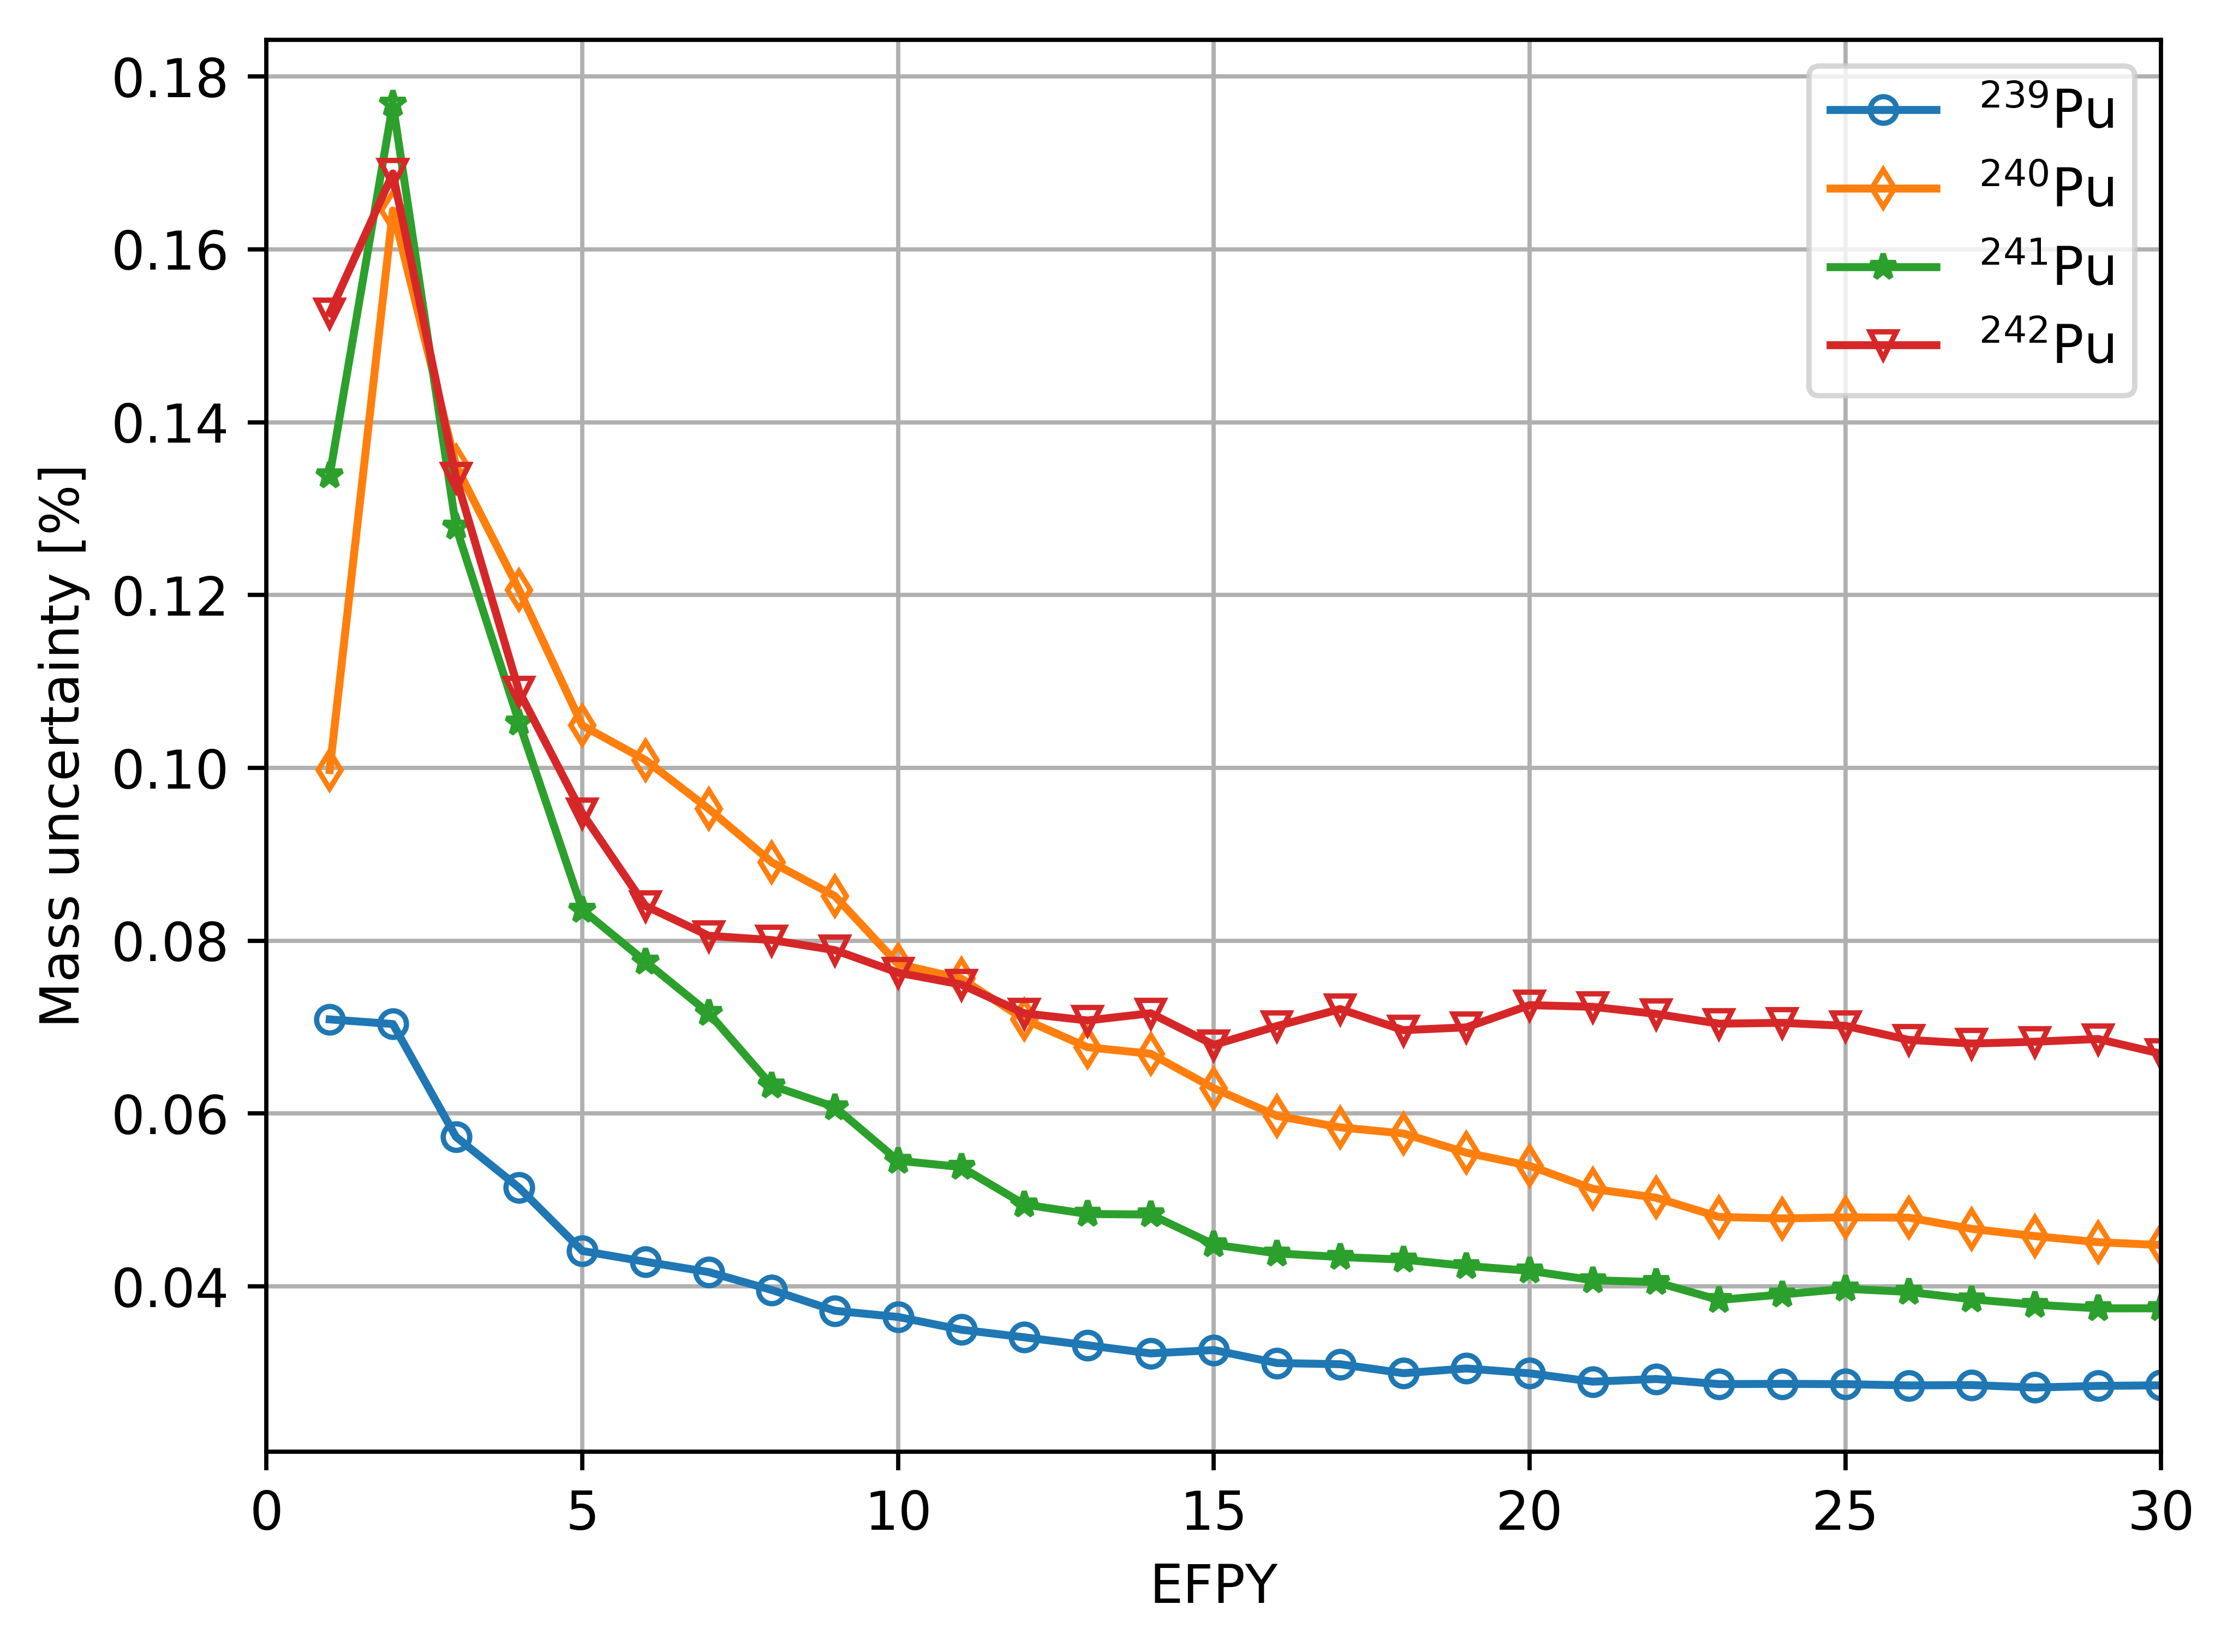
\includegraphics[width=0.8\textwidth]{uq/serpent_mass_std_pu.png}
	\caption{Caption here.}
	\label{fig:pu}
\end{figure}
\begin{figure}[hbp!] % replace 't' with 'b' to 
	\centering
	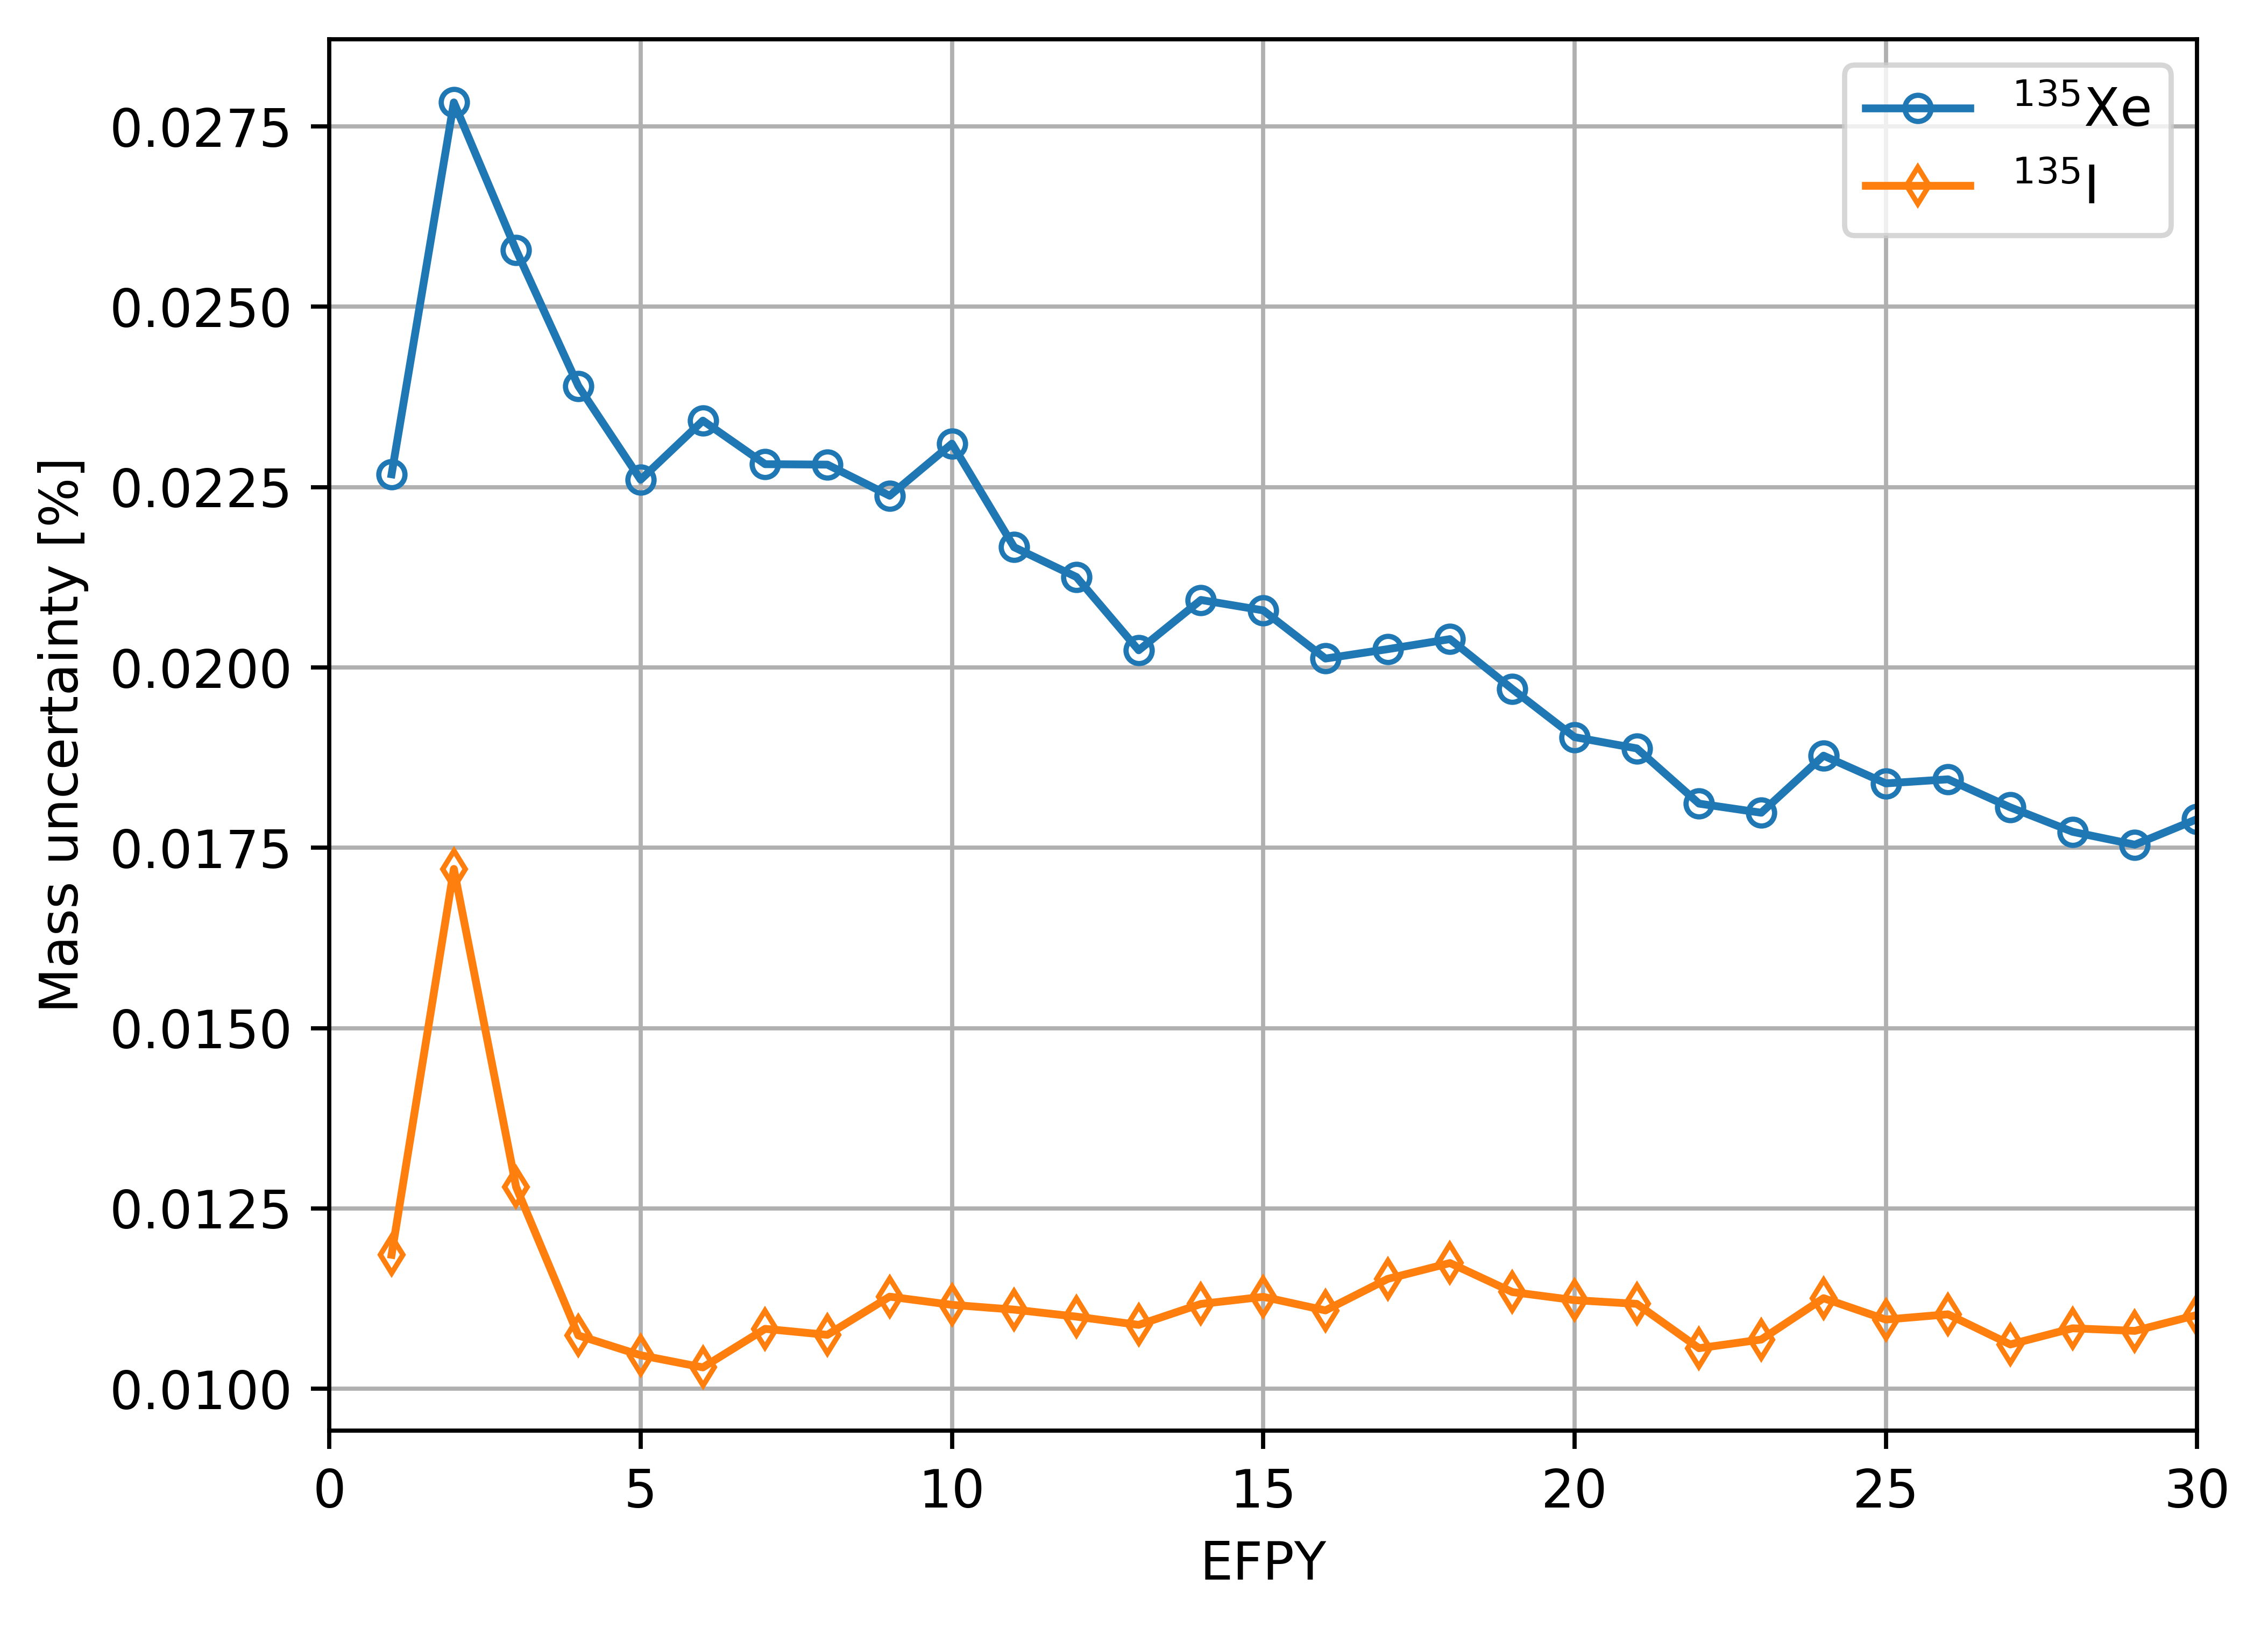
\includegraphics[width=0.8\textwidth]{uq/serpent_mass_std_xe_i.png}
	\caption{Caption here.}
	\label{fig:xe-i}
\end{figure}
\begin{figure}[hbp!] % replace 't' with 'b' to 
	\centering
	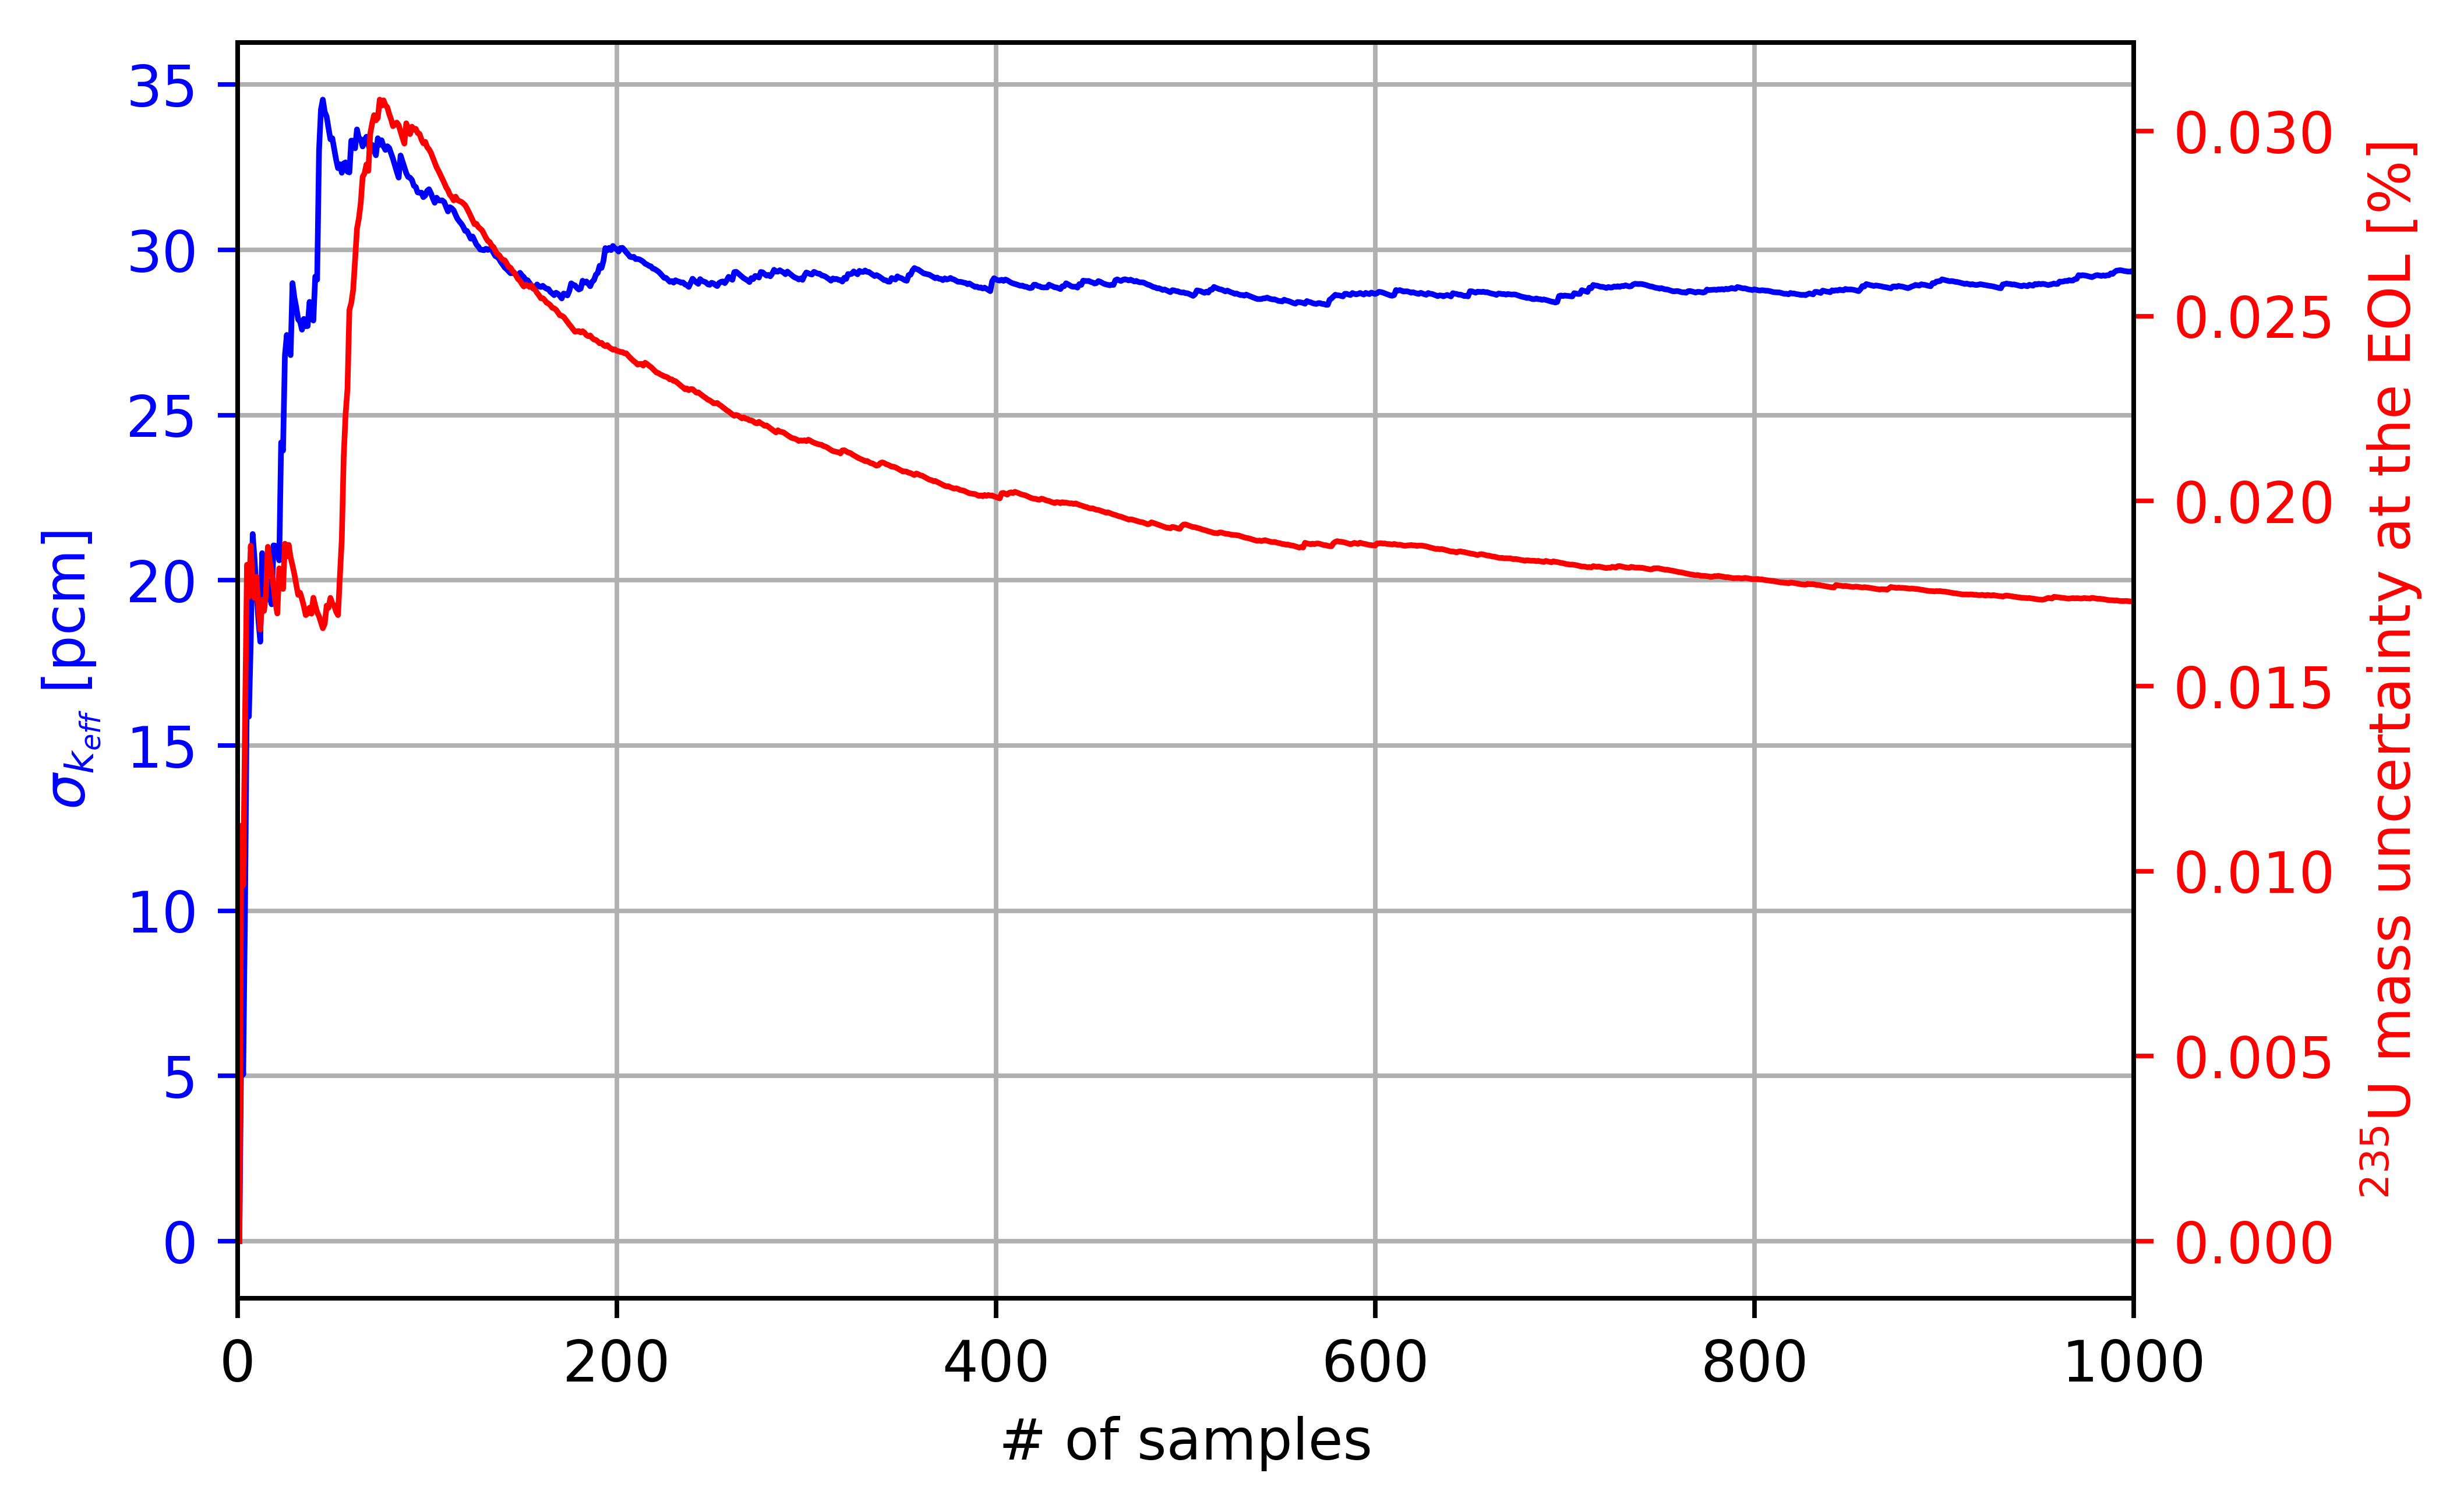
\includegraphics[width=0.8\textwidth]{uq/serpent_convergance_for_tap.png}
	\caption{Caption here.}
	\label{fig:uq-convergance}
\end{figure}

\section{Nuclear data related uncertainty in depleted fuel composition}

\begin{figure}[hbp!] % replace 't' with 'b' to 
	\centering
	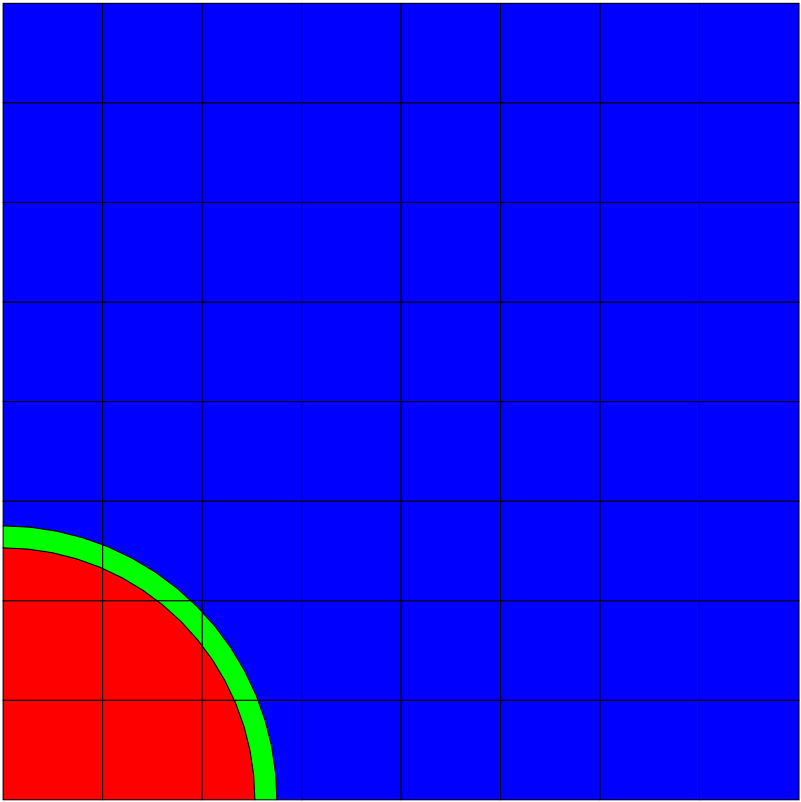
\includegraphics[width=0.8\textwidth]{uq/tap_pin_for_scale.png}
	\caption{Caption here.}
	\label{fig:uq-tap-pincell}
\end{figure}
\begin{figure}[hbp!] % replace 't' with 'b' to 
	\centering
	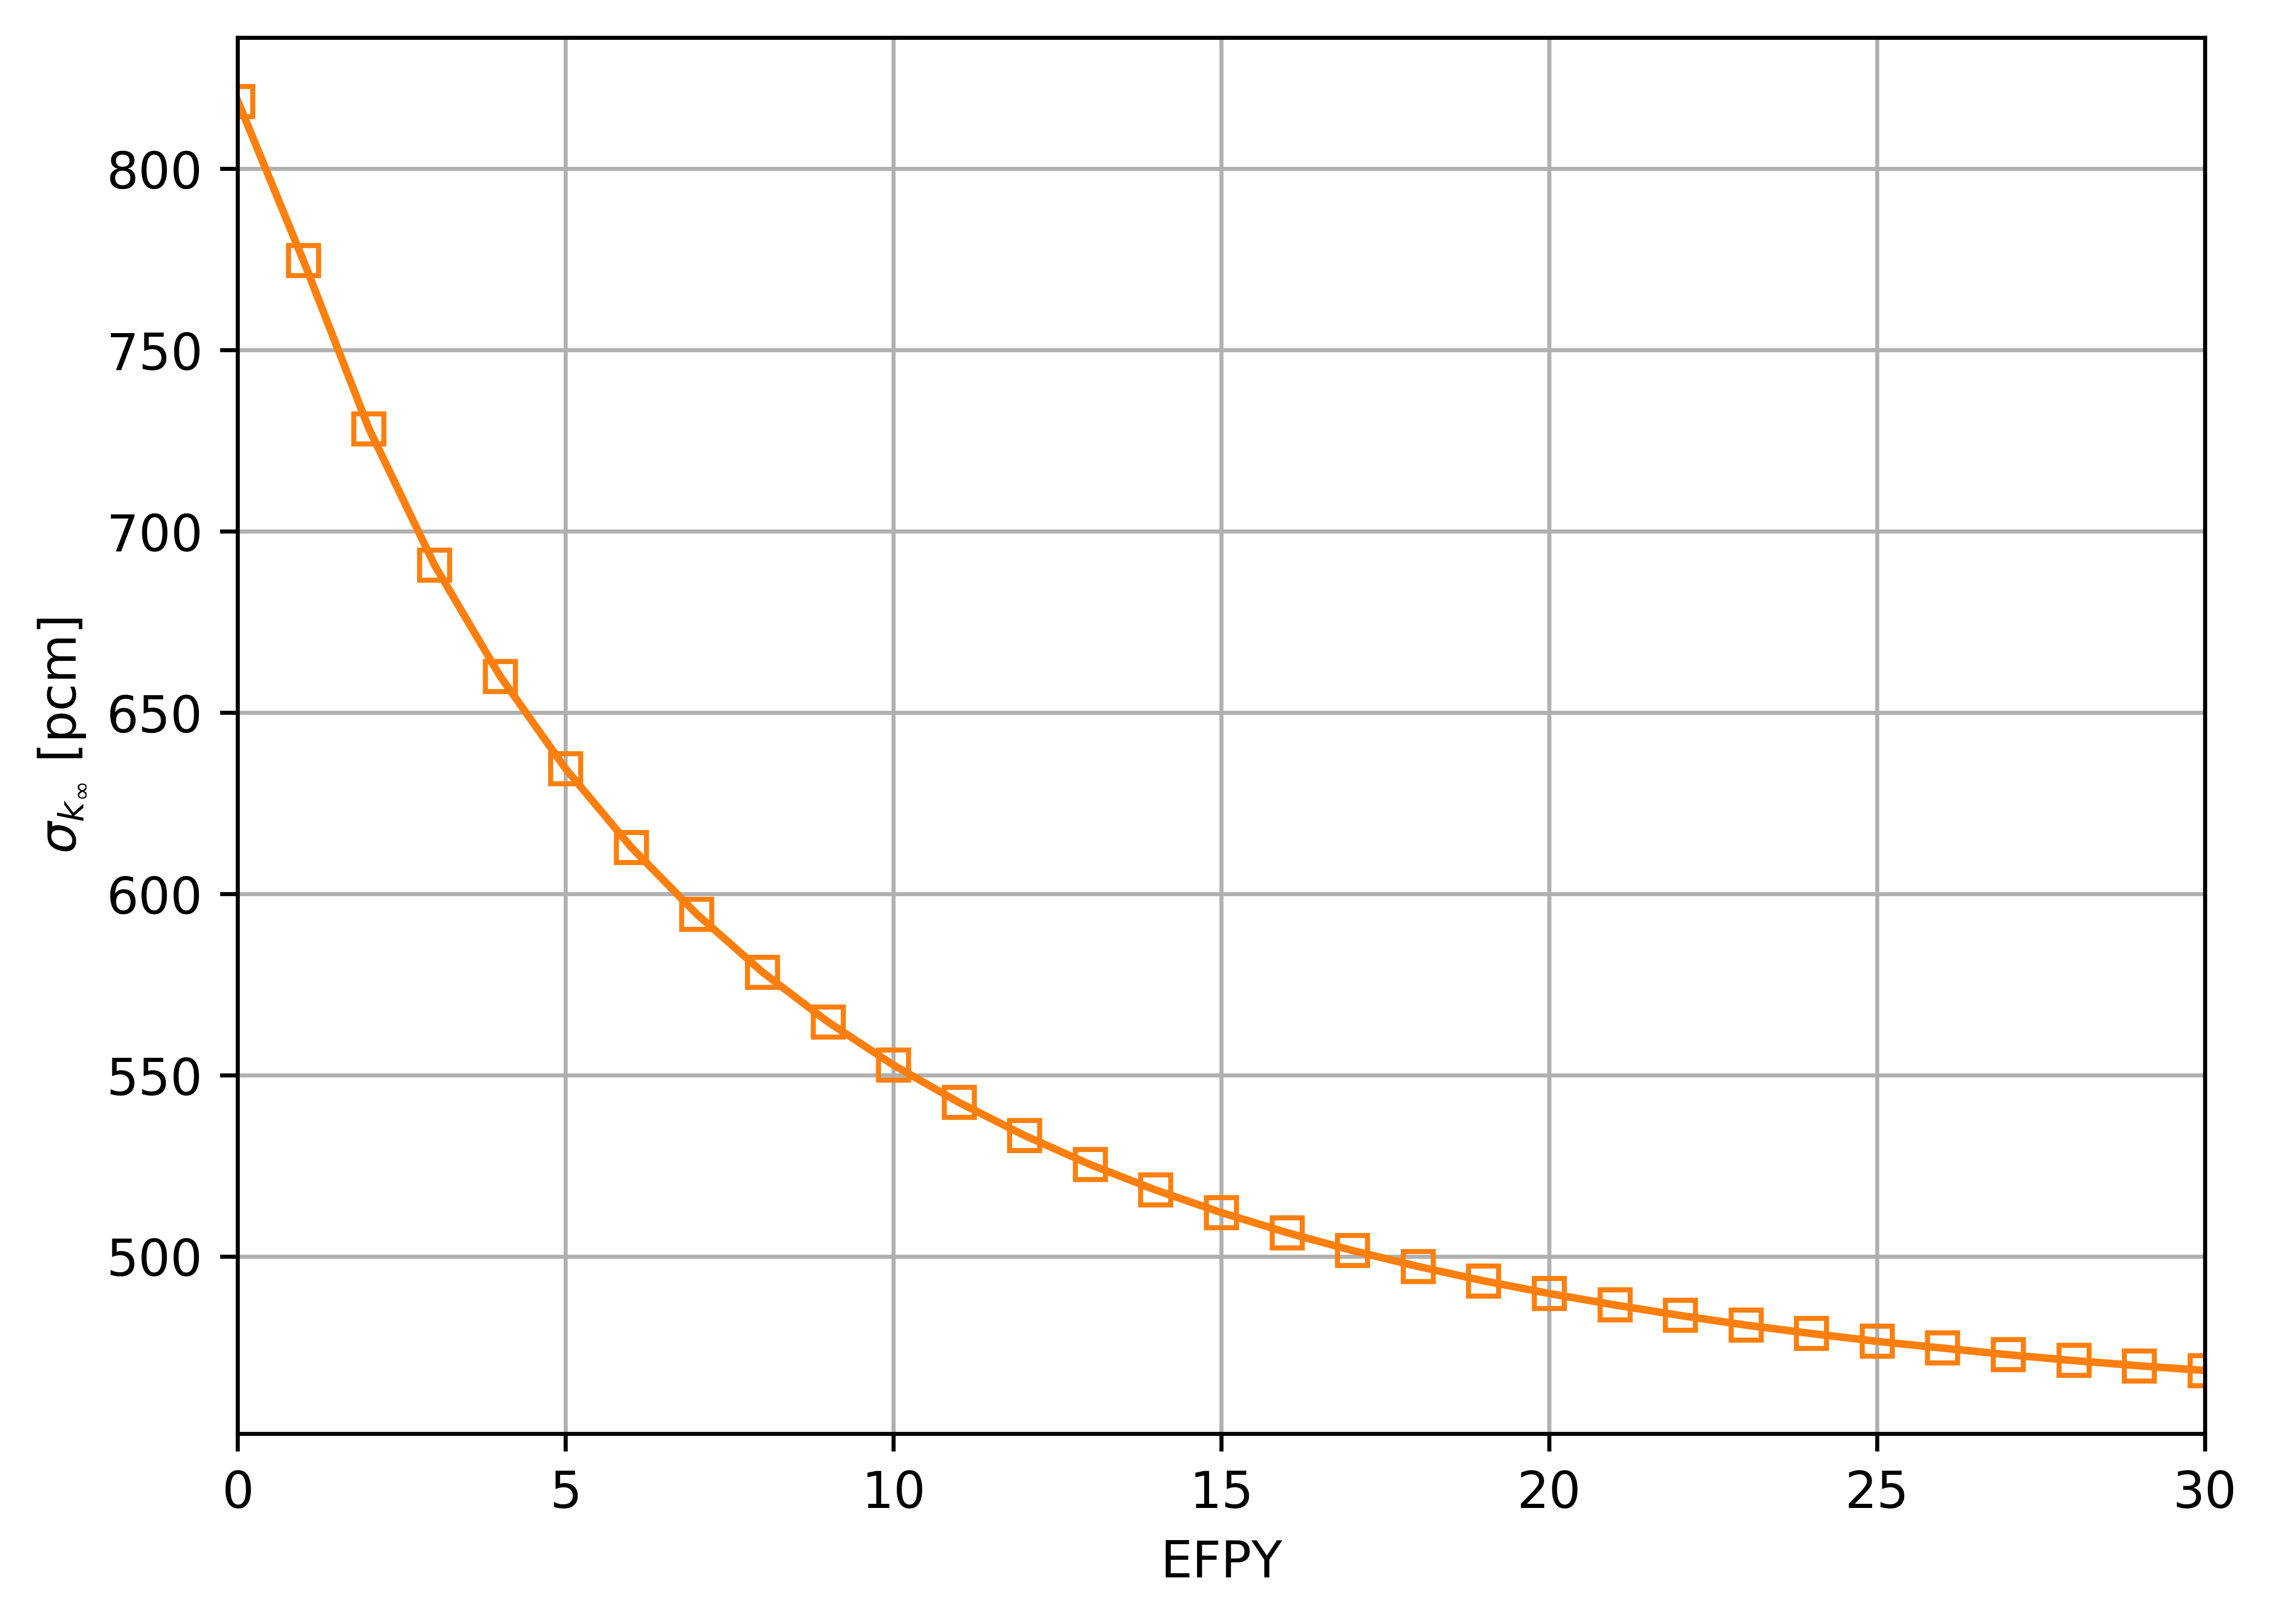
\includegraphics[width=0.8\textwidth]{uq/scale_kinf_dynamics_for_tap.png}
	\caption{Caption here.}
	\label{fig:uq-scale-kinf}
\end{figure}
\begin{figure}[hbp!] % replace 't' with 'b' to 
	\centering
	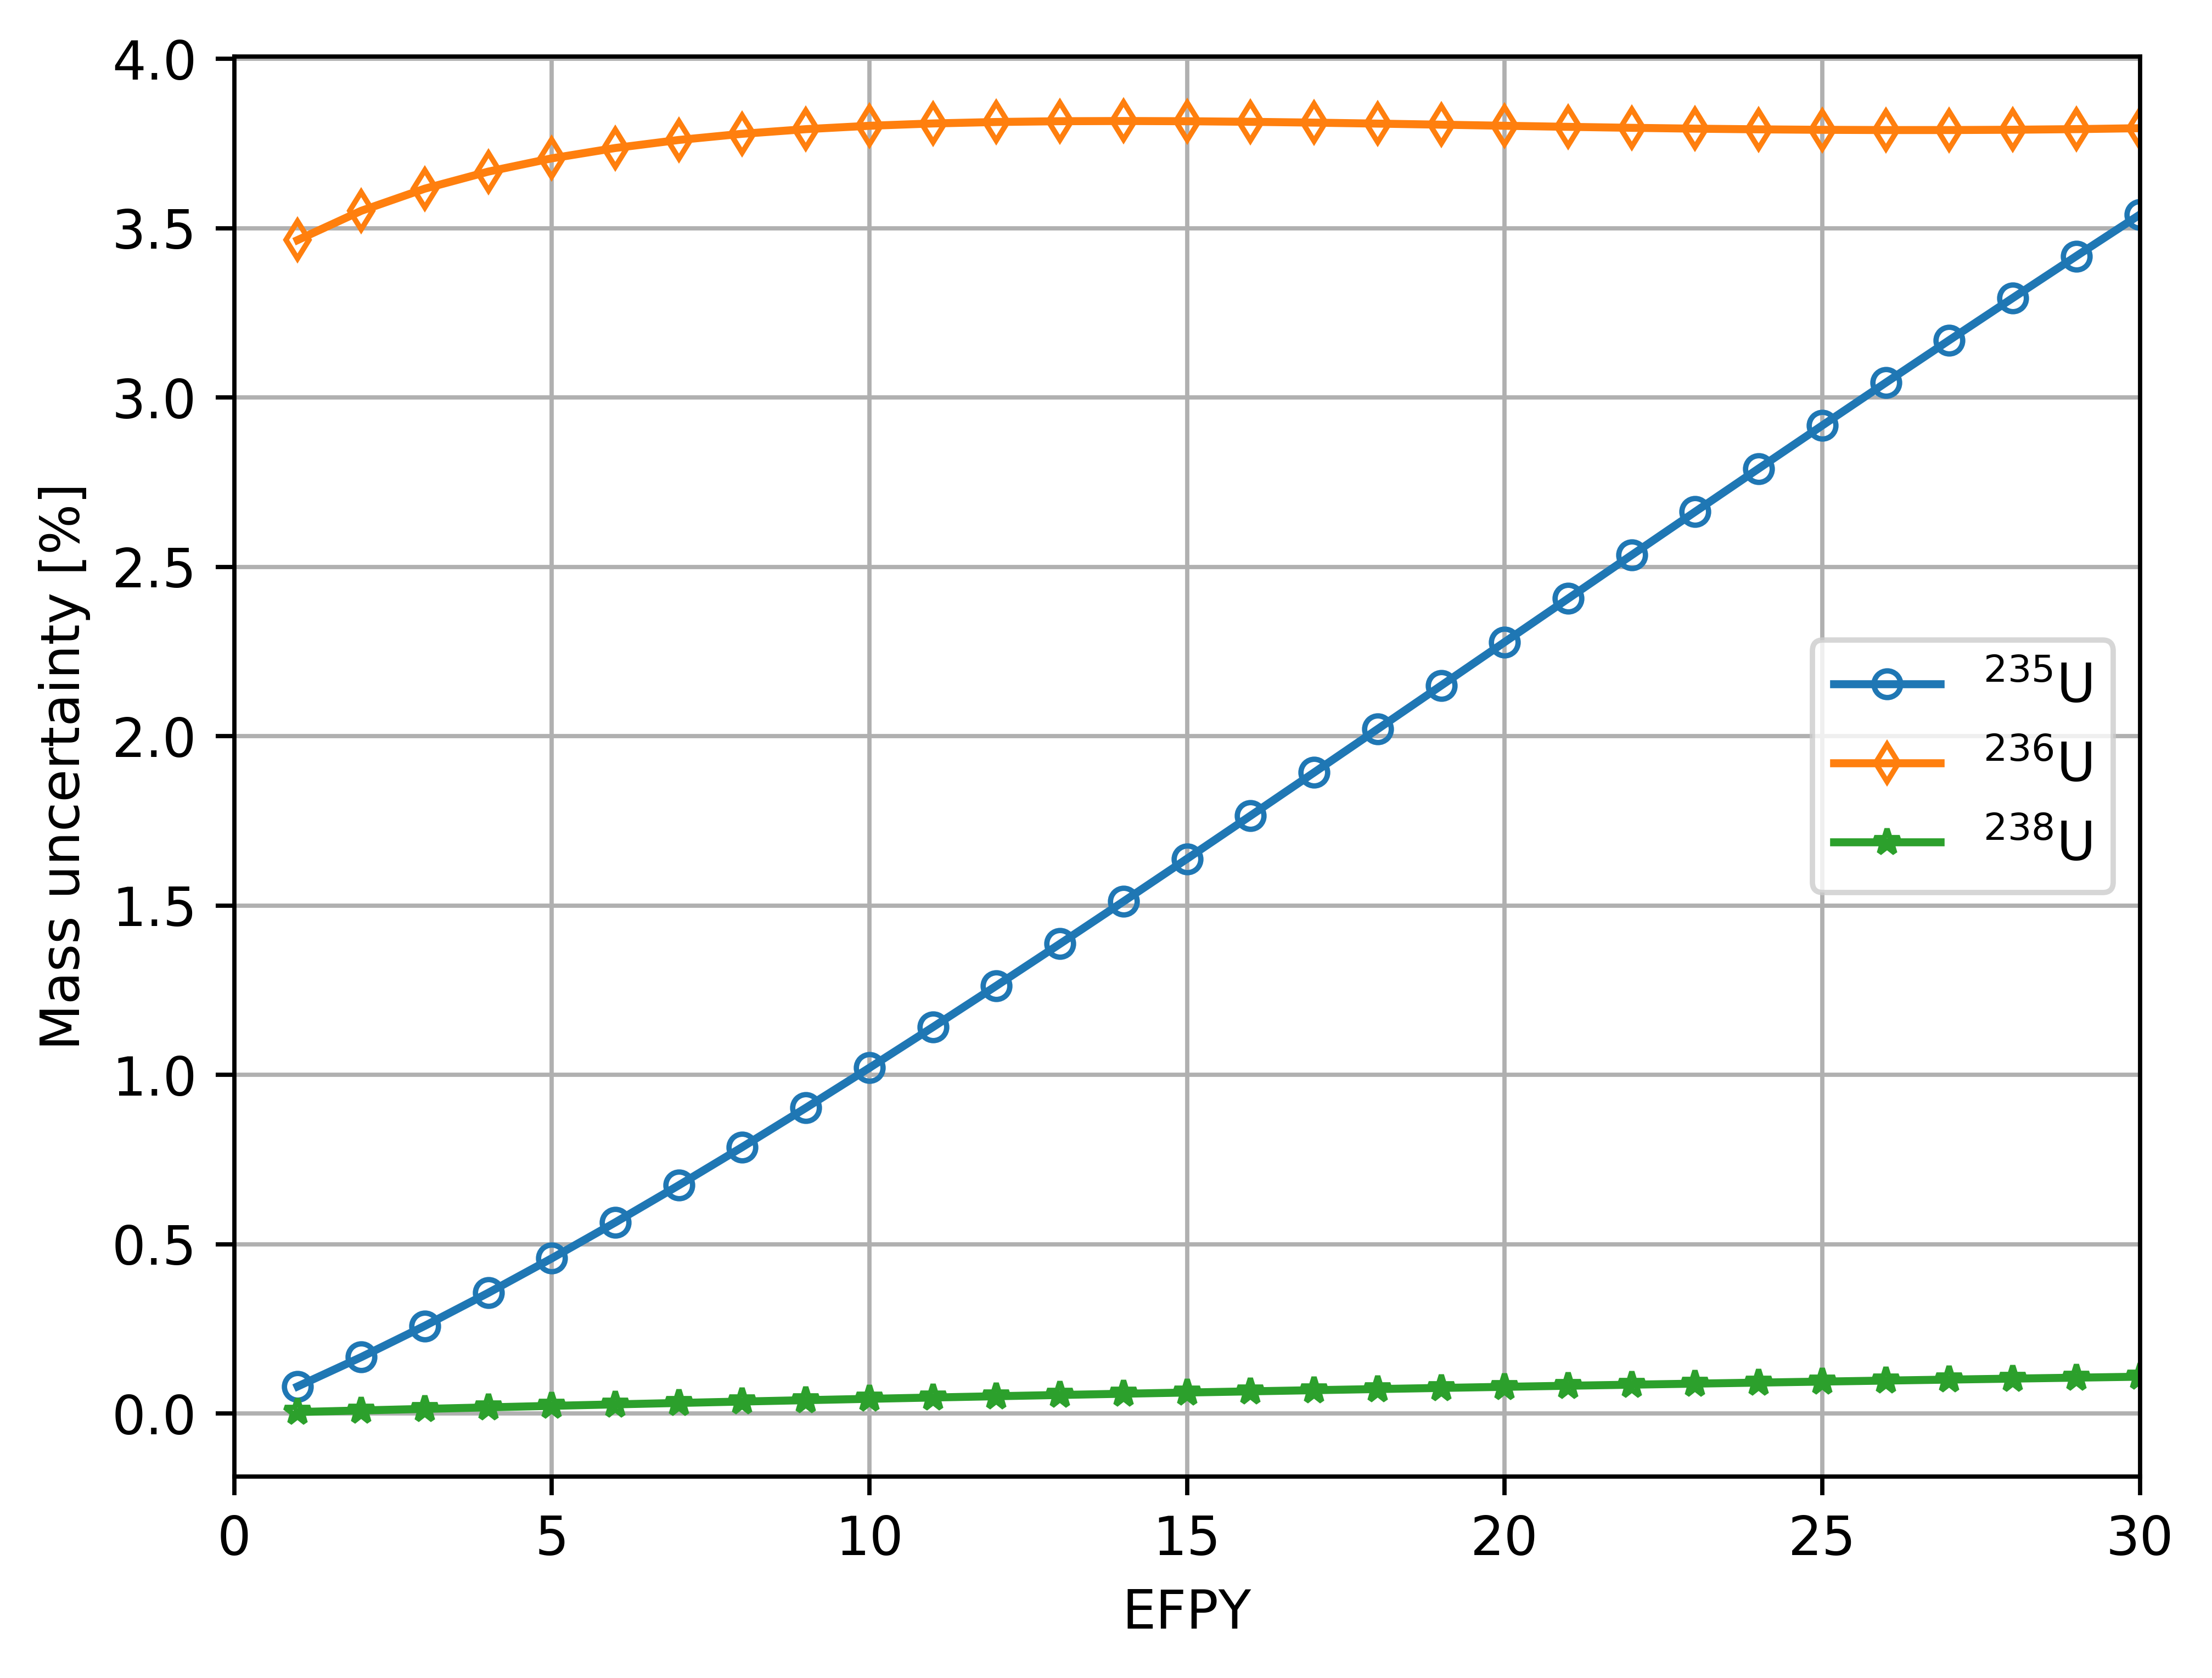
\includegraphics[width=0.8\textwidth]{uq/scale_mass_std_u.png}
	\caption{Caption here.}
	\label{fig:uq-scale-u}
\end{figure}

\begin{figure}[hbp!] % replace 't' with 'b' to 
	\centering
	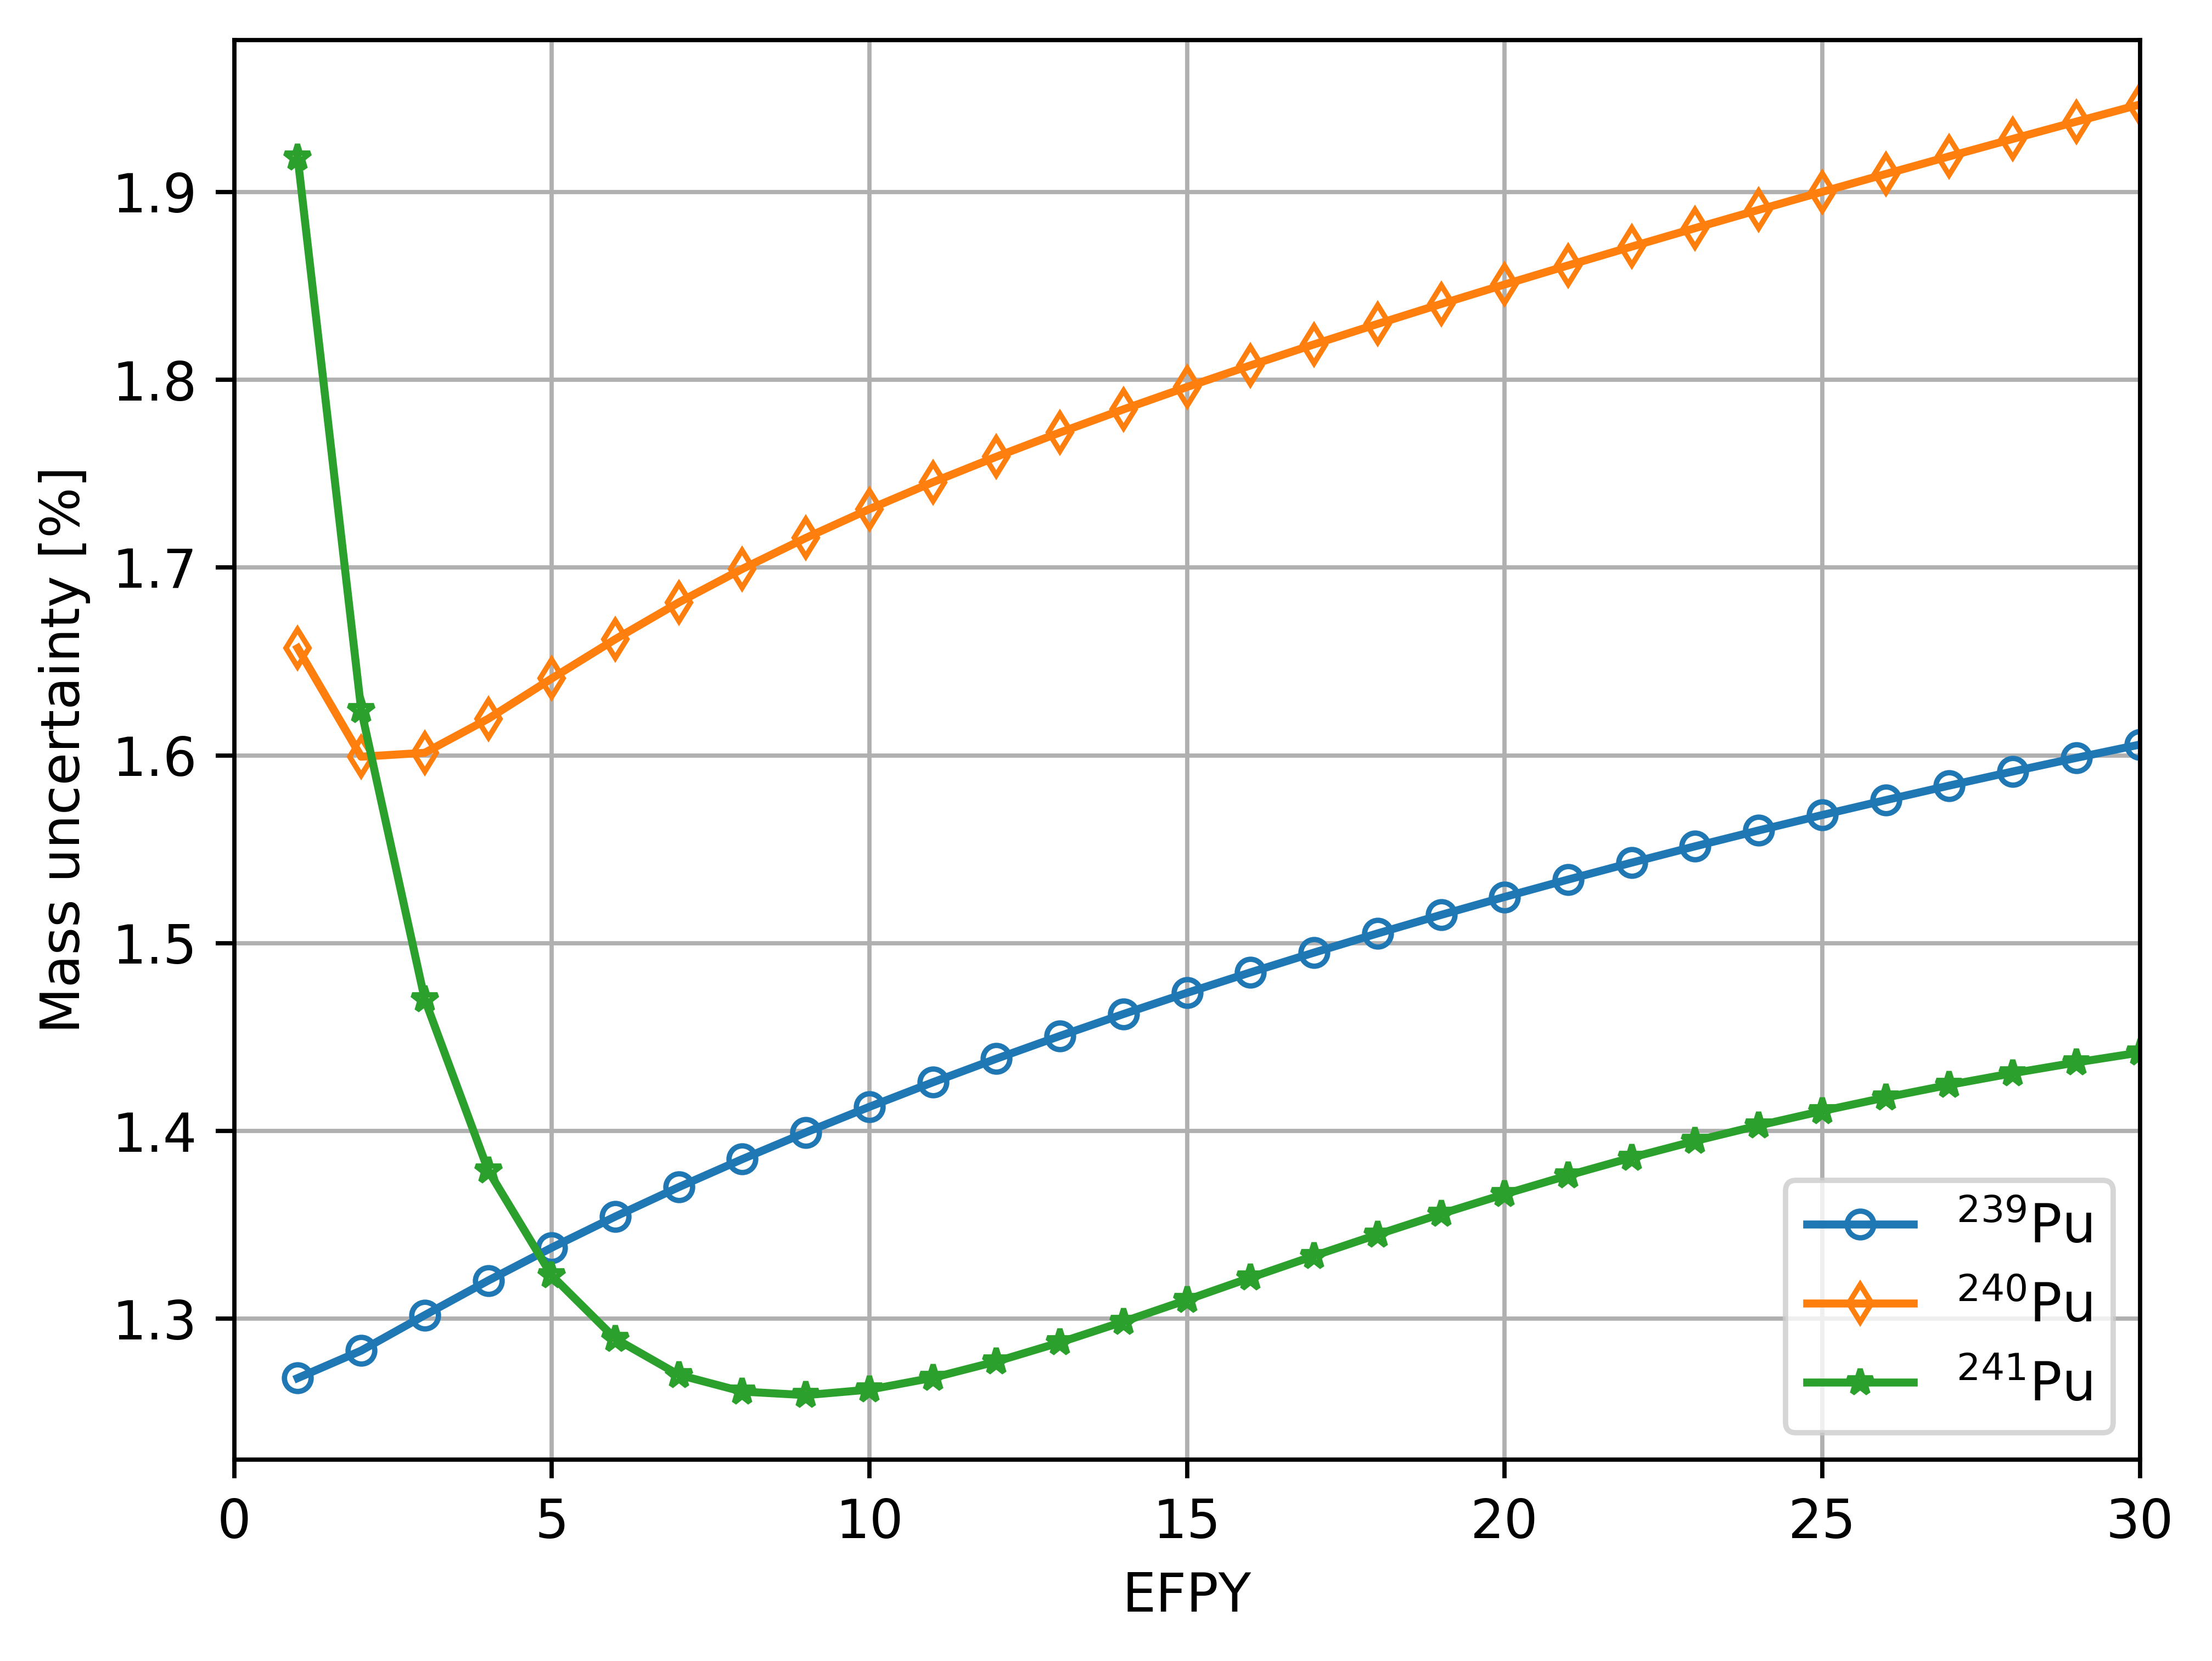
\includegraphics[width=0.8\textwidth]{uq/scale_mass_std_pu.png}
	\caption{Caption here.}
	\label{fig:uq-scale-pu}
\end{figure}
\begin{figure}[hbp!] % replace 't' with 'b' to 
	\centering
	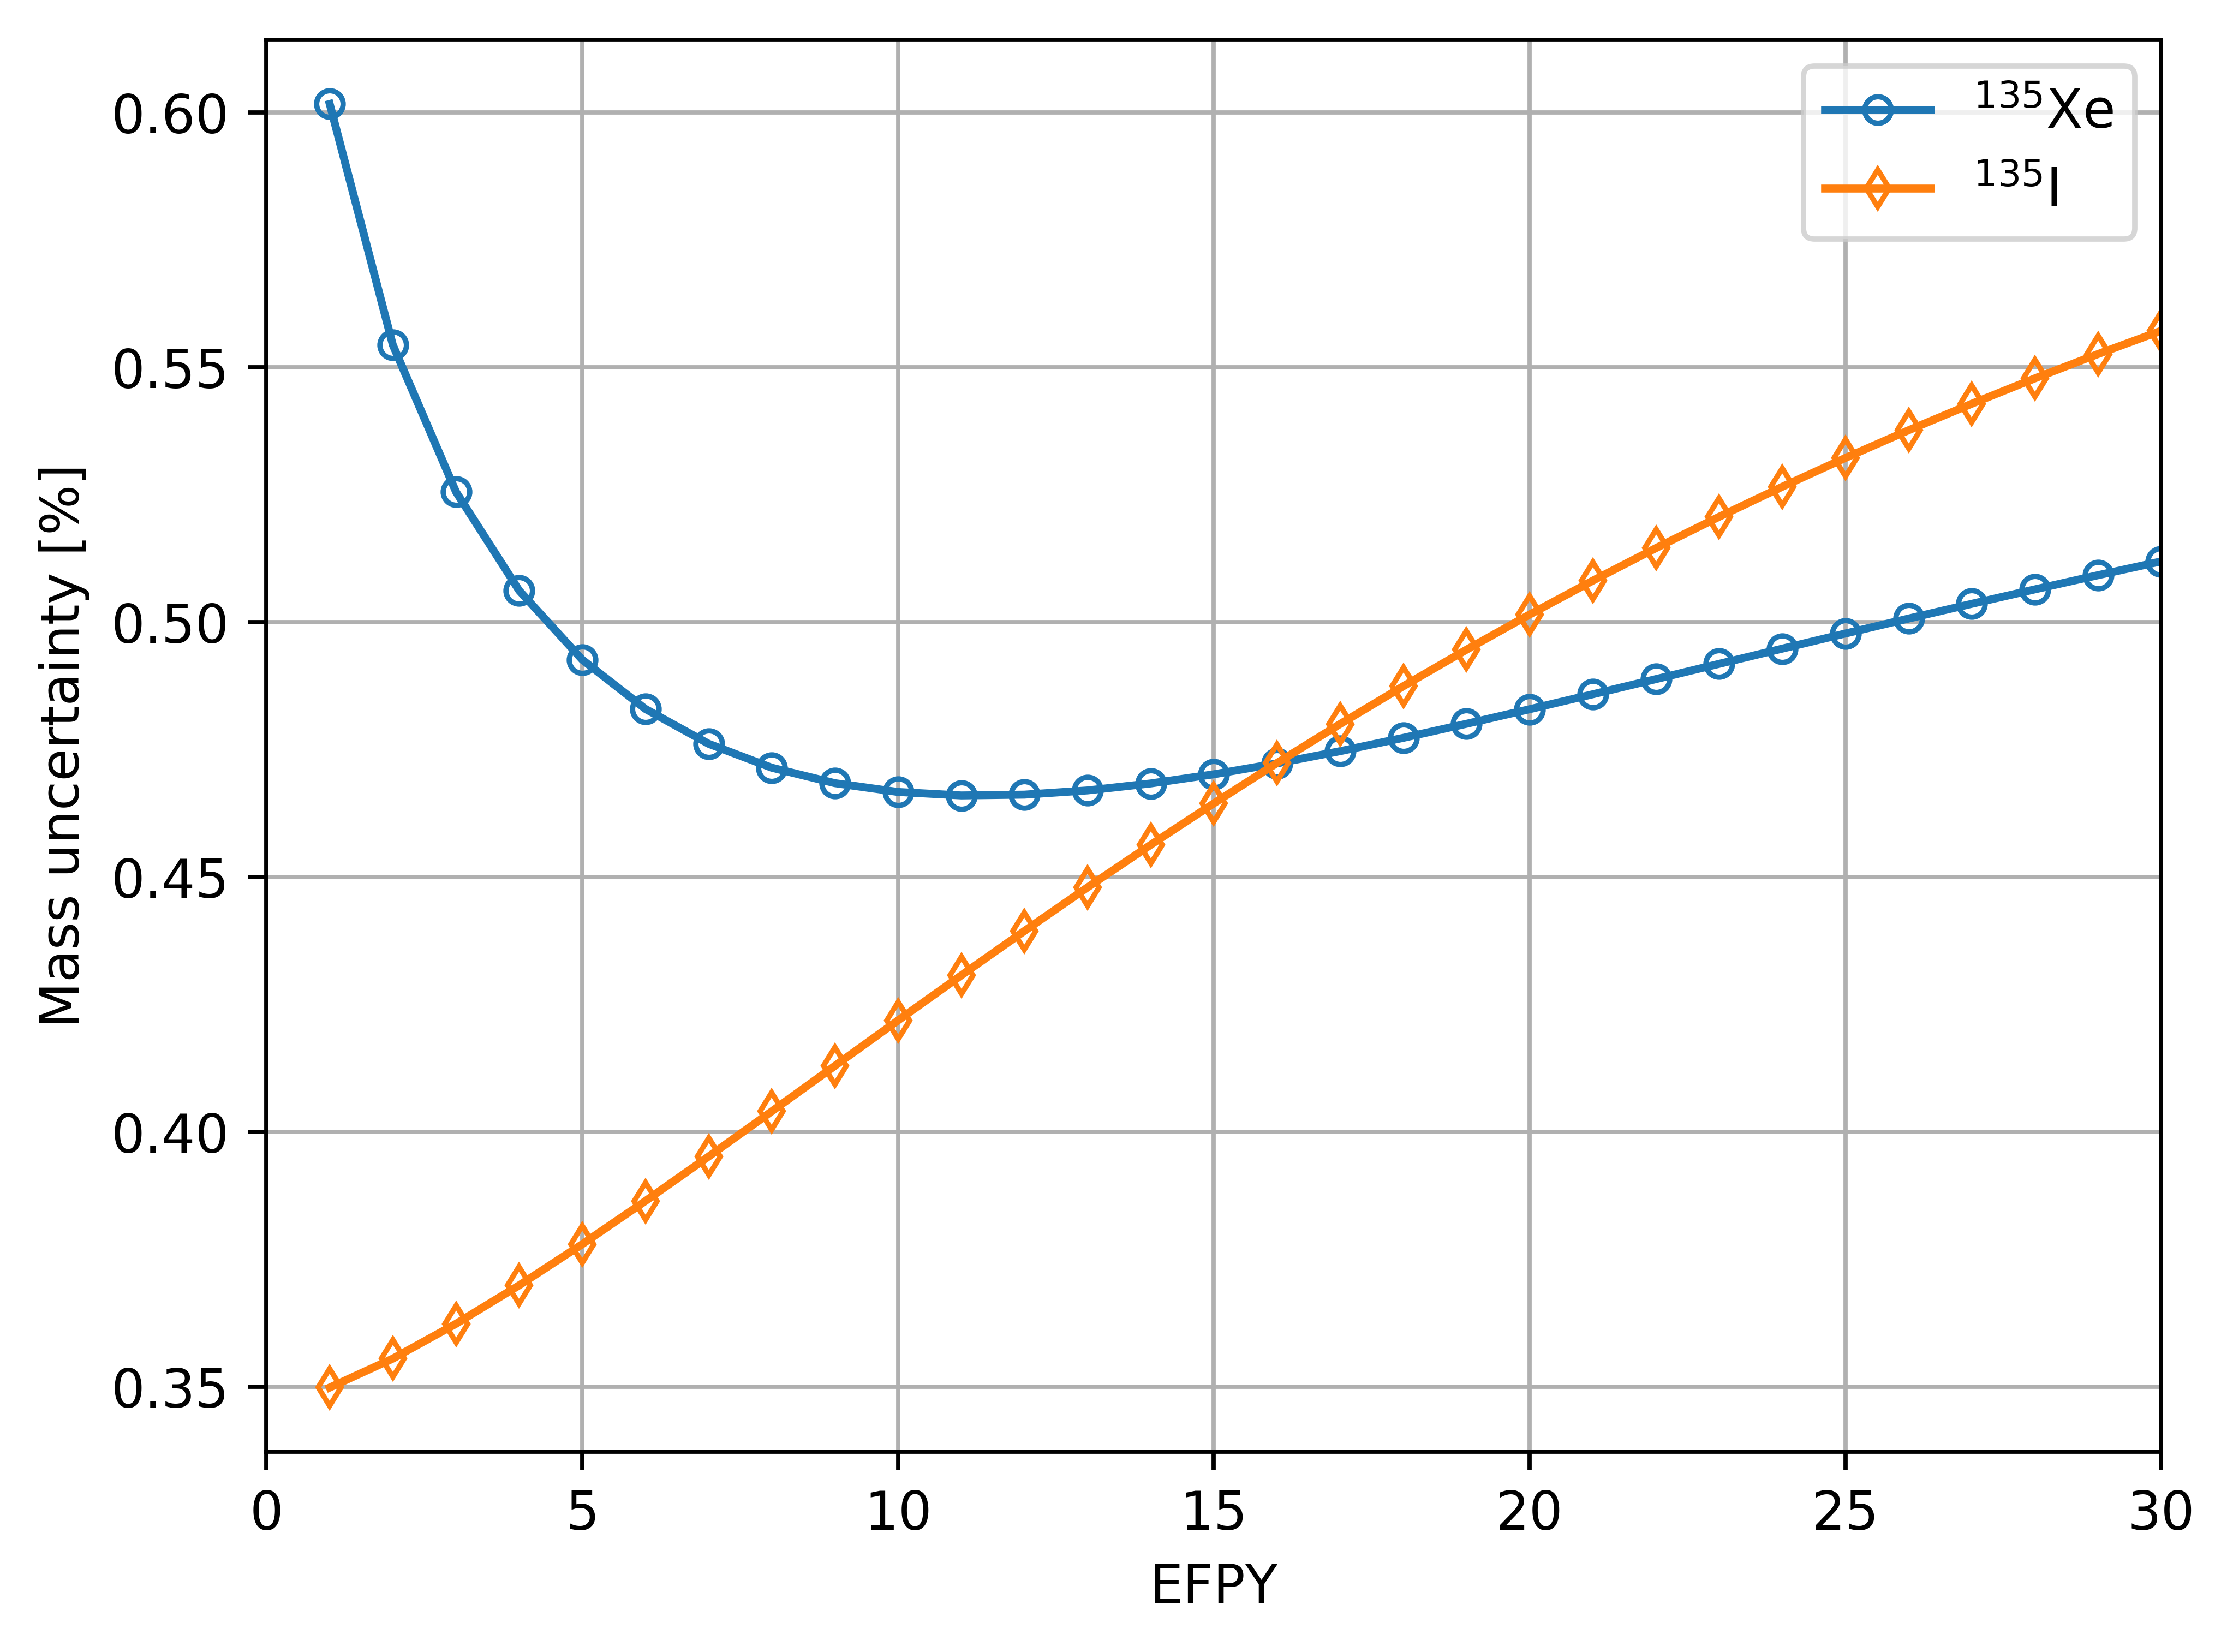
\includegraphics[width=0.8\textwidth]{uq/scale_mass_std_xe_i.png}
	\caption{Caption here.}
	\label{fig:uq-scale-xe-i}
\end{figure}
\begin{figure}[hbp!] % replace 't' with 'b' to 
	\centering
	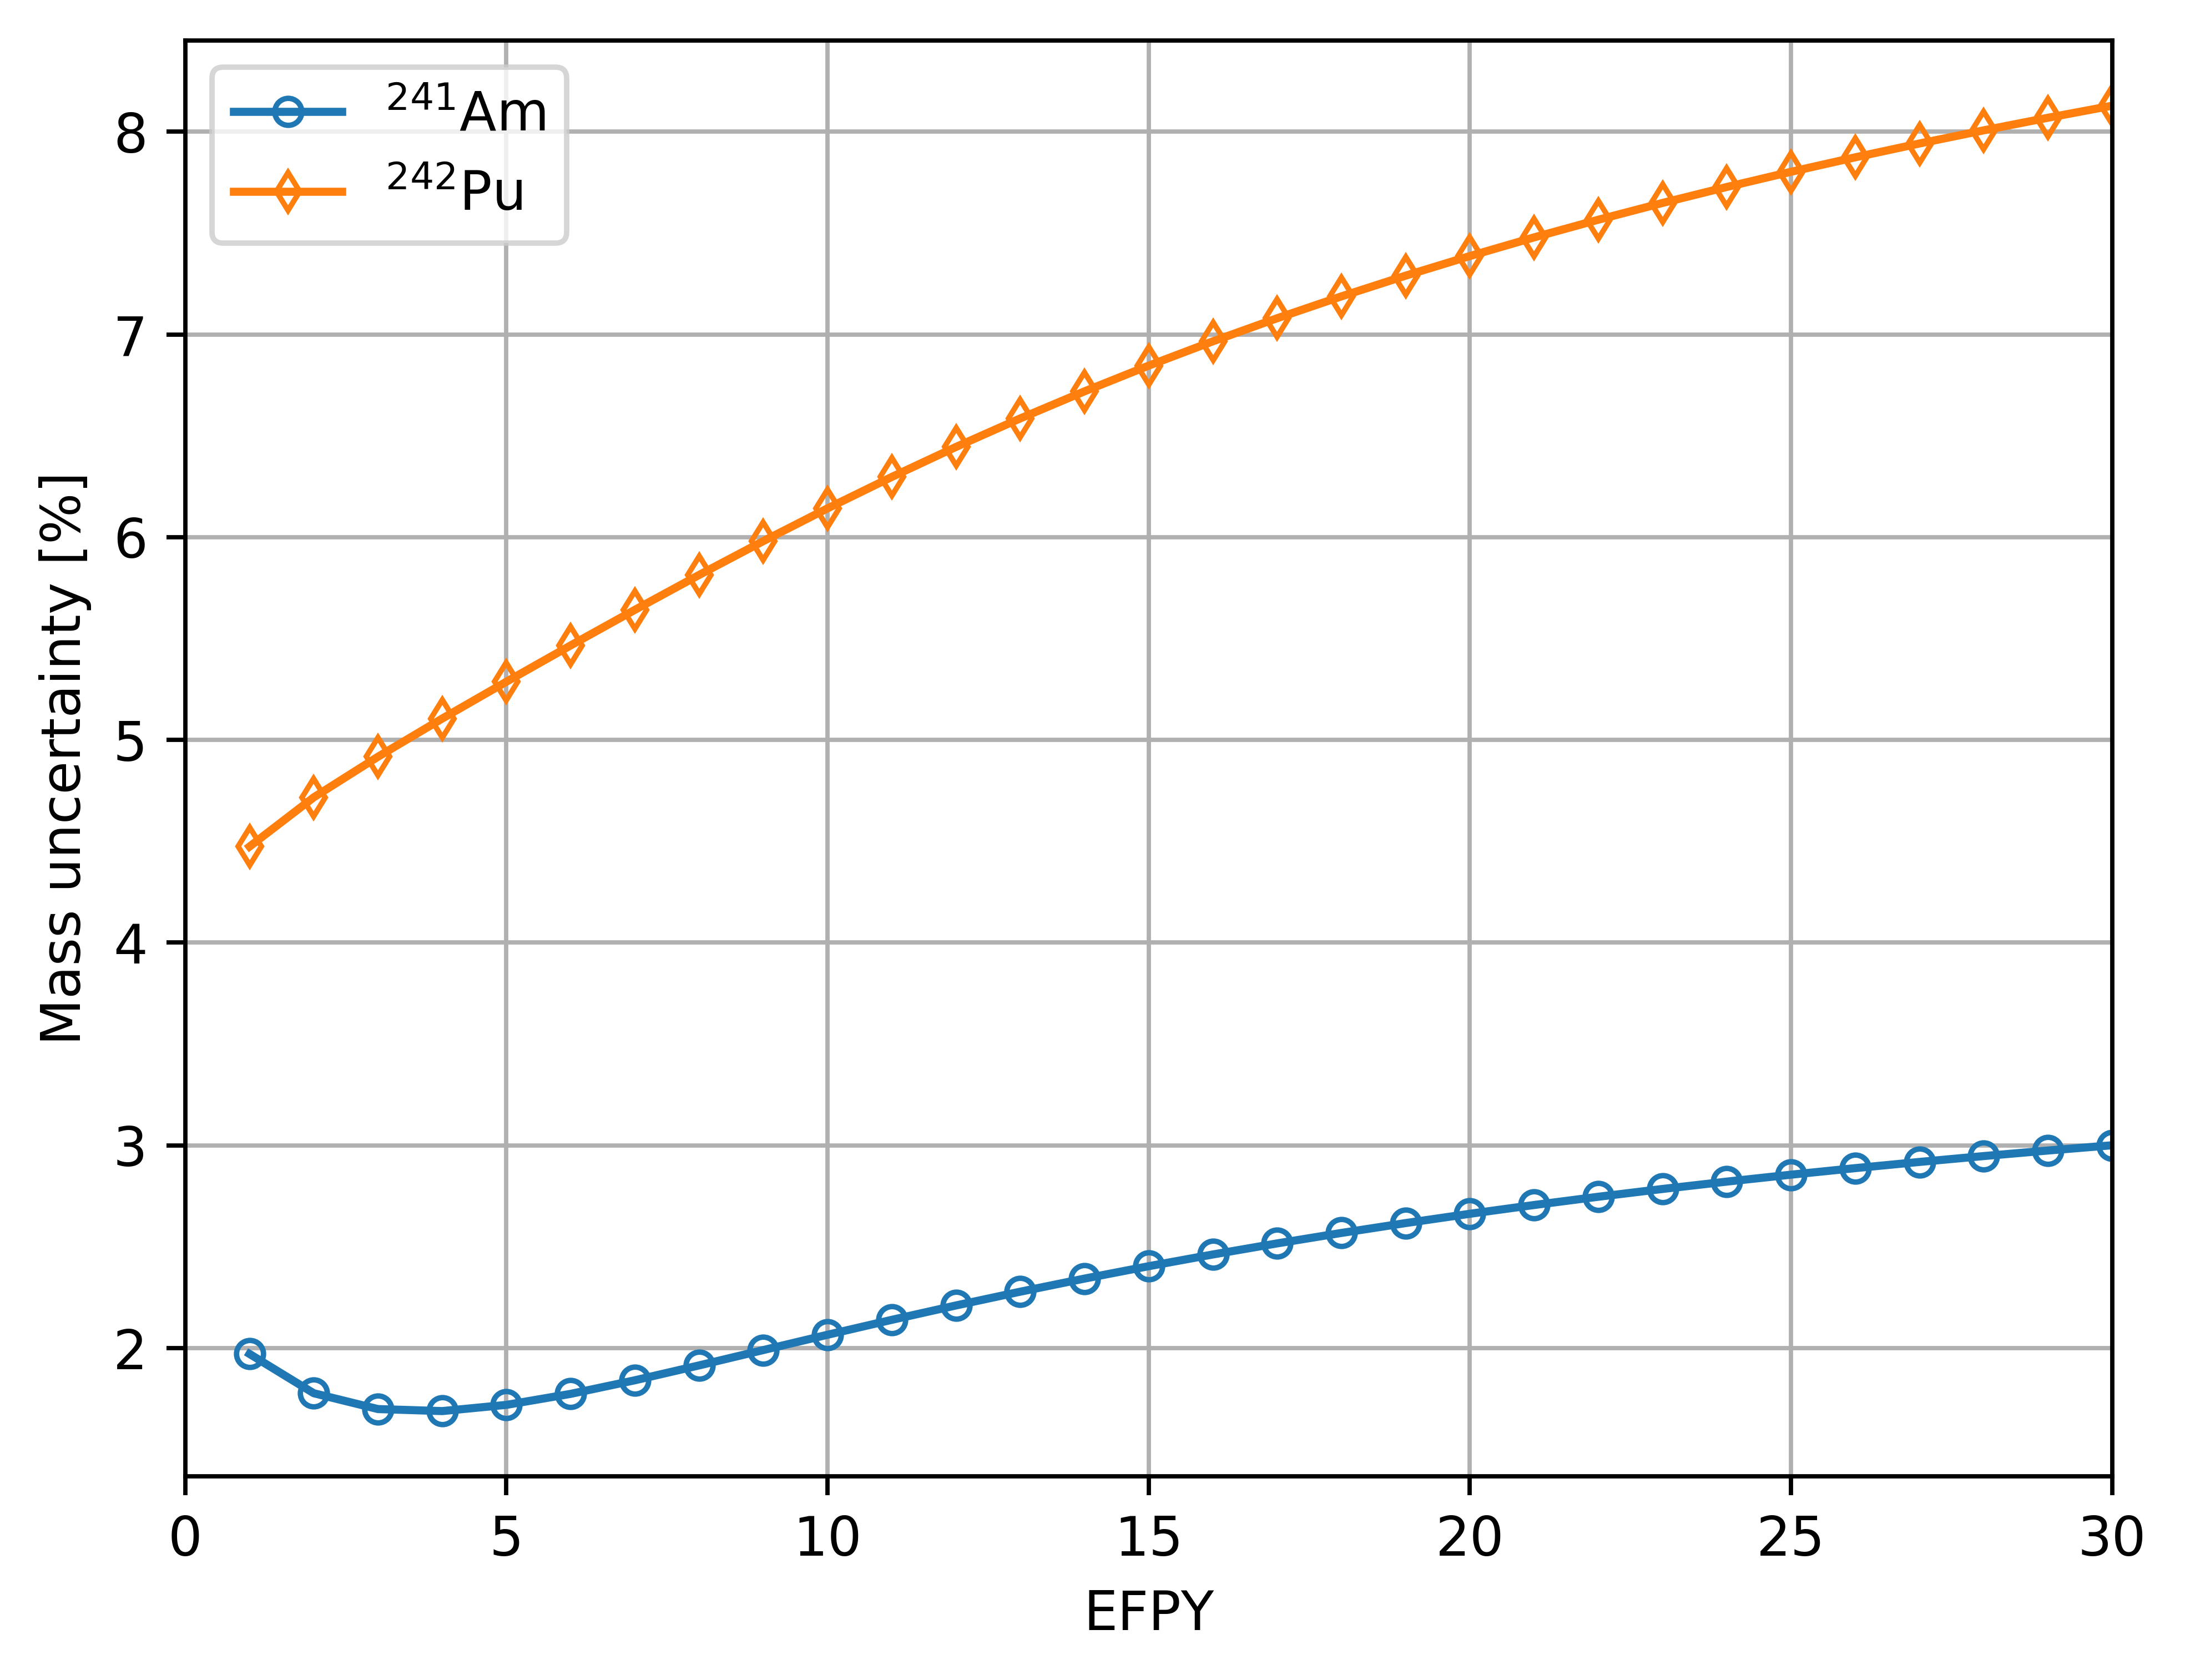
\includegraphics[width=0.8\textwidth]{uq/scale_mass_std_act.png}
	\caption{Caption here.}
	\label{fig:uq-scale-act}
\end{figure}

\begin{figure}[hbp!] % replace 't' with 'b' to 
	\centering
	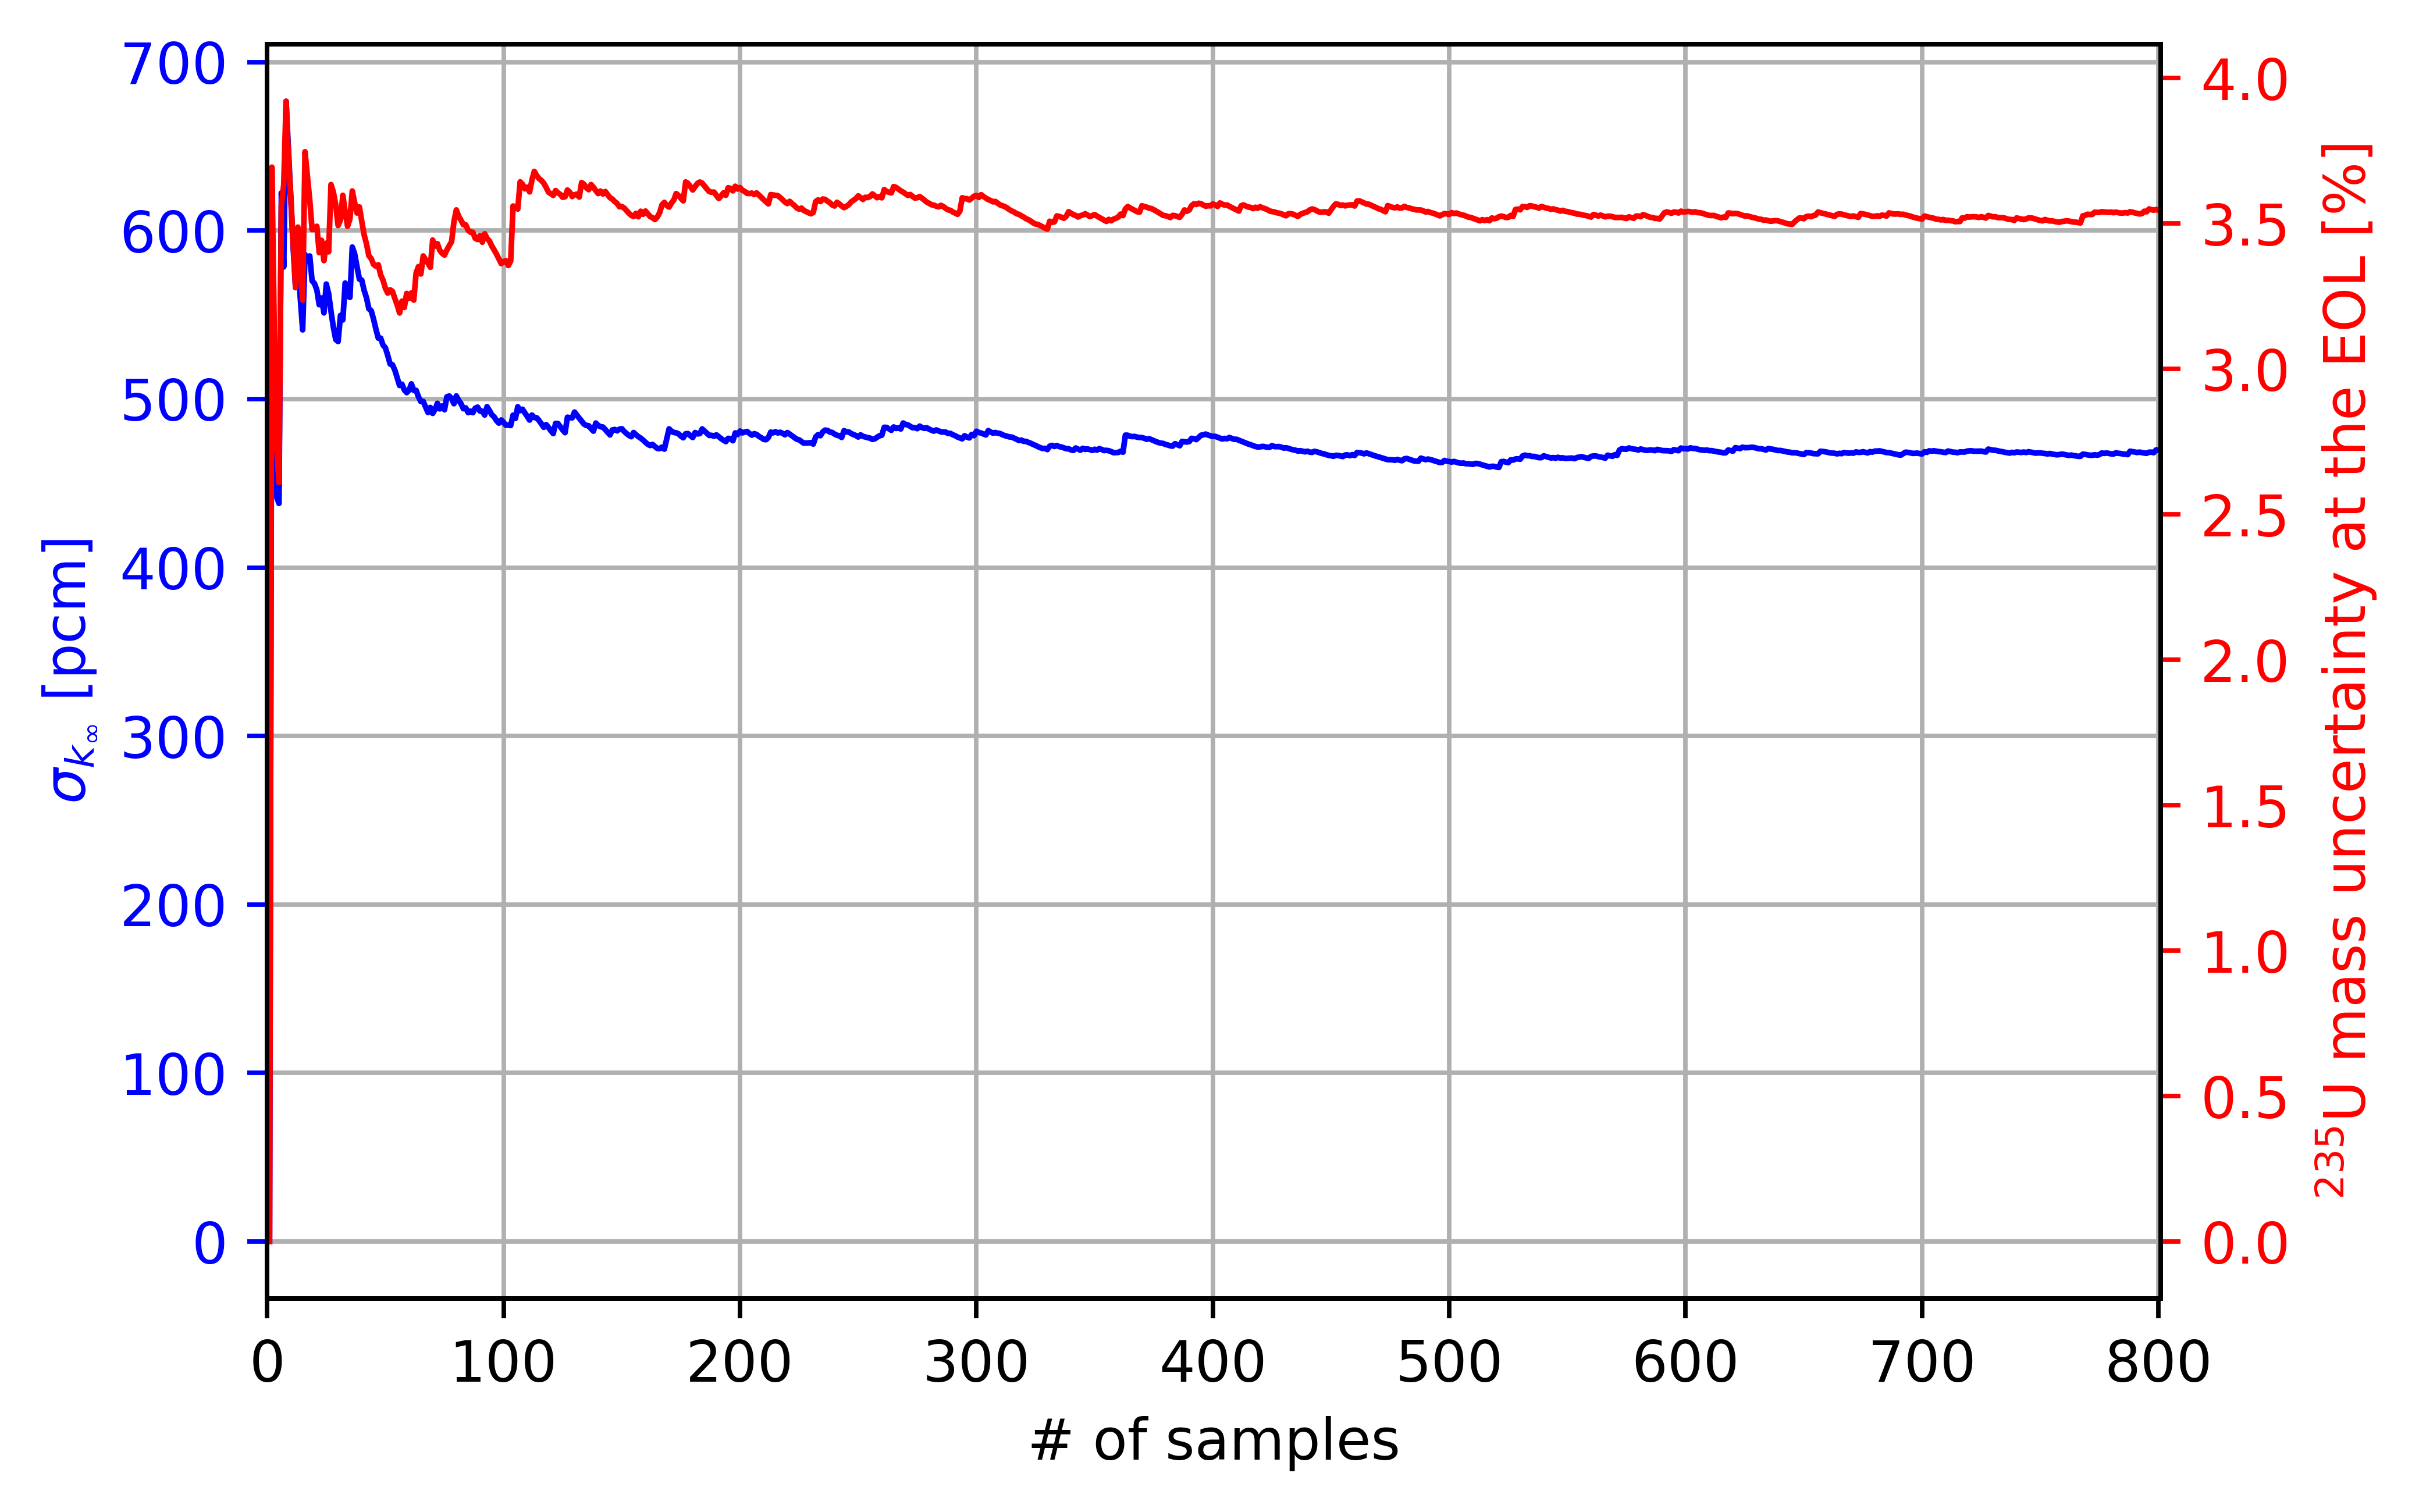
\includegraphics[width=0.8\textwidth]{uq/scale_convergance_for_tap.png}
	\caption{Caption here.}
	\label{fig:uq-scale-convergance}
\end{figure}

\section{Concluding remarks}